% Created 2022-05-18 Wed 14:21
% Intended LaTeX compiler: pdflatex
\documentclass[12pt, reqno, oneside]{amsbook}
              \newcommand\subtitle[1]{\newcommand\mrgsubtitle{#1}}
\newcommand\mrgproject{}
\newcommand\mrgtitle{Torsten: A Pharmacokinetic/Pharmacodynamic Model Library for Stan}
\newcommand\mrgsubtitle{\large{User's Guide} \linebreak (Torsten Version 0.91.0, Stan version 2.33.1)}
\include{mrgtitlepage}
\usepackage{imakeidx}
\makeindex
\usepackage[letterpaper, width=6.5in, height=9in]{geometry}
\usepackage{graphicx}
\usepackage{pdfpages}
\usepackage{amssymb}
\usepackage{epstopdf}
\usepackage{xcolor}
\definecolor{MRGGreen}{rgb}{0, 0.350, 0.200}
\usepackage[colorlinks=true, citecolor=MRGGreen, urlcolor=MRGGreen, linkcolor=MRGGreen]{hyperref}
\usepackage{bold-extra}
\usepackage{courier}
\usepackage{listings}
% \usepackage{siunitx}
\usepackage{booktabs}
\usepackage[framemethod=TikZ, skipabove=10pt, skipbelow=10pt, backgroundcolor=black!3, roundcorner=4pt, linewidth=1pt]{mdframed}
\BeforeBeginEnvironment{minted}{\begin{mdframed}}
\AfterEndEnvironment{minted}{\end{mdframed}}
\usepackage{subcaption}
\renewcommand{\chaptername}{}
\numberwithin{equation}{chapter}
\numberwithin{figure}{chapter}
\numberwithin{table}{chapter}
\usepackage[section]{placeins}
\renewcommand{\thesection}{\thechapter.\arabic{section}}
\theoremstyle{remark}
\newtheorem{example}{Example}
\newtheorem{remark}{Remark}


\usepackage[utf8]{inputenc}
\usepackage[T1]{fontenc}
\usepackage{graphicx}
\usepackage{grffile}
\usepackage{longtable}
\usepackage{wrapfig}
\usepackage{rotating}
\usepackage[normalem]{ulem}
\usepackage{amsmath}
\usepackage{textcomp}
\usepackage{amssymb}
\usepackage{capt-of}
\usepackage[newfloat]{minted}
\usemintedstyle{xcode}          % avoid red boxes in minted blocks
\usepackage{caption}
\setcounter{secnumdepth}{3}
\author{Yi Zhang}
\date{\today}
\title{Torsten: A Pharmacokinetic/Pharmacodynamic Model Library for Stan\\\medskip
\large User's Guide \\  (Torsten Version 0.91.0, Stan version 2.33.1)}
\hypersetup{
 pdfauthor={Yi Zhang},
 pdftitle={Torsten: A Pharmacokinetic/Pharmacodynamic Model Library for Stan},
 pdfkeywords={},
 pdfsubject={},
 pdfcreator={Emacs 28.1 (Org mode 9.4.4)},
 pdflang={English}}
\begin{document}

\maketitle
\tableofcontents


\chapter*{Development team}
\label{sec:org5ae31e5}
\begin{itemize}
\item \href{mailto:billg@metrumrg.com}{William R. Gillespie} , \href{https://www.metrumrg.com/}{Metrum Research Group}
\item \href{mailto:yz@yizh.org}{Yi Zhang} , \href{https://www.c-path.org/}{Critical Path Institute}
\item \href{mailto:cmargossian@flatironinstitute.org}{Charles Margossian} , Flatiron Institute
\end{itemize}
\chapter*{Acknowledgements}
\label{sec:orgab46cef}
\section*{Institutions}
\label{sec:orgb690148}
We thank Metrum Research Group, Columbia University, and AstraZeneca.
\section*{Funding}
\label{sec:org1bad1f4}
This work was funded in part by the following organizations:
\subsection*{Office of Naval Research (ONR) contract N00014-16-P-2039}
\label{sec:org228195e}
provided as part of the Small Business Technology Transfer (STTR)
program. The content of the information presented in this document
does not necessarily reflect the position or policy of the
Government and no official endorsement should be inferred.
\subsection*{Bill \& Melinda Gates Foundation.}
\label{sec:orga901041}
\section*{Individuals}
\label{sec:org87098de}
We thank the Stan Development Team for giving us guidance on how to
create new Stan functions and adding features to Stan's core language
that facilitate building ODE-based models.

We also thank Kyle Baron and Hunter Ford for helpful advice on coding
in C++ and using GitHub, Curtis Johnston for reviewing the User
Manual, and Yaming Su for using Torsten and giving us feedback.
\chapter{Introduction}
\label{sec:orgc21e46a}
\href{https://mc-stan.org/}{Stan} is an open source probabilistic programing language designed
primarily to do Bayesian data analysis
\cite{carpenter17_stan}. It provides an expressive syntax for statistic
modeling and contains an efficient variant of No U-Turn
Sampler(NUTS), an adaptative Hamiltonian Monte Carlo
algorithm that was proven more efficient than commonly used Monte Carlo Markov Chains
(MCMC) samplers for complex high dimensional problems \cite{hoffman_no-u-turn_2011,betancourt_hmc_2018}.

Torsten is a collection of Stan functions to facilitate analysis of
pharmacometric data. Given an event schedule and an ODE system, it calculates amounts
in each compartment. The current version includes \footnote{\textbf{WARNING:} The current version of Torsten is a \emph{prototype}. It is being released for review and comment, and to support limited research applications. It has not been rigorously tested and should not be used for critical applications without further testing or cross-checking by comparison with other methods. We encourage interested users to try Torsten out and are happy to assist. Please report issues, bugs, and feature requests on \href{https://github.com/metrumresearchgroup/stan}{our GitHub page}.}:
\begin{itemize}
\item Specific linear compartment models:
\begin{itemize}
\item One compartment model with first order absorption.
\item Two compartment model with elimination from and first order absorption into central compartment
\end{itemize}
\item General linear compartment model described by a system of first-order \uline{linear} Ordinary Differential Equations (ODEs).
\item General compartment model described by a system of first order ODEs.
\item Coupled model with PK forcing function described by a linear one or two compartment model and PD components solved by numerical ODE integration.
\end{itemize}

The models and data format are based on
NONMEM \textregistered{} \footnote{NONMEM\textregistered{} is licensed and distributed by ICON Development Solutions.}/NMTRAN/PREDPP
conventions including:
\begin{itemize}
\item recursive calculation of model predictions, which permits piecewise constant covariate values,
\item bolus or constant rate inputs into any compartment,
\item single dose and multiple dose events,
\item steady state dosing events,
\item NMTRAN-compartible data items such as TIME, EVID, CMT, AMT, RATE, ADDL, II, and SS.
\end{itemize}

All real variable arguments in Torsten functions can be passed as Stan \texttt{parameters}.

\section{Implementation summary}
\label{sec:orgabe7e42}
\begin{itemize}
\item Current Torsten v0.91.0 is based on Stan v2.33.1.
\item All functions are programmed in C++ and are compatible
with the Stan math automatic differentiation library \cite{carpenter15_stan_math_librar}
\item One and two compartment models are based on analytical solutions of governing ODEs.
\item General linear compartment models are based on semi-analytical solutions using the built-in matrix exponential function
\item General compartment models are solved numerically using built-in ODE integrators in Stan. The tuning parameters of the solver are adjustable. The steady state solution is calculated using a numerical algebraic solver.
\item Coupled model that has PK forcing function solved analytically and PD ODE components solved numerically.
\end{itemize}

\section{Development plans}
\label{sec:org8ee92bb}
Our current plans for future development of Torsten include the
following:
\begin{itemize}
\item Build a system to easily share packages of Stan functions
(written in C++ or in the Stan language)
\item Optimize Matrix exponential functions
\begin{itemize}
\item Function for the action of Matrix Exponential on a vector
\item Hand-coded gradients
\item Special algorithm for matrices with special properties
\end{itemize}
\item Develop new method for large-scale hierarchical models with costly
ODE solving.
\item Fix issue that arises when computing the adjoint of the lag time
parameter (in a dosing compartment) evaluated at \(t_{\text{lag}} = 0\).
\item Extend formal tests
\begin{itemize}
\item More unit tests and better CD/CI support.
\item Comparison with simulations from the R package
\texttt{mrgsolve} and the software NONMEM\textregistered{}
\item Recruit non-developer users to conduct beta testing
\end{itemize}
\end{itemize}

\chapter{Changelog}
\label{sec:org6ee814c}
\begin{itemize}
  \item Version 0.91.1 \textit{<2024-12-01 Sun>}
\begin{itemize}
\item Changed
\begin{itemize}
\item More model examples fixes.
\item Remove ODE group integrator functions.
\item Improve documentation.
\end{itemize}
\end{itemize}
\item Version 0.91.0 \textit{<2023-12-31 Sun>}
\begin{itemize}
\item Changed
\begin{itemize}
\item Update model examples according to new array syntax.
\item Update to Stan version 2.33.1.
\item Removed experimental cross-chain feature.
\item Deprecation of old Torsten functions not using 'pmx\_' prefix.
\end{itemize}
\end{itemize}
\item Version 0.90.0 \textit{<2022-05-18 Wed>}
\begin{itemize}
\item Changed
\begin{itemize}
\item Update model examples according to new array syntax.
\item Update to Stan version 2.29.2.
\end{itemize}
\end{itemize}
\item Version 0.89 \textit{<2021-06-15 Tue>}
\begin{itemize}
\item Changed
\begin{itemize}
\item New backend for ODE events solvers.
\item Use vector instead of array as ODE function state \& return type.
\item Simplified ODE integrator naming, e.g. \texttt{pmx\_ode\_bdf[\_ctrl]}.
\item Update to Stan version 2.27.0.
\end{itemize}
\end{itemize}
\item Version 0.88 \textit{<2020-12-18 Fri>}
\begin{itemize}
\item Added
\begin{itemize}
\item Bioavailability, lag time, ODE real \& integer data are optional in PMX function signatures.
\item Support all EVID options from NM-TRAN and mrgsolve.
\item Support steady-state infusion through multiple interdose intervals.
\end{itemize}
\end{itemize}

\begin{itemize}
\item Changed
\begin{itemize}
\item More efficient memory management of COVDES implenmentation.
\item Update of MPI framework to adapt multilevel paralleism.
\item Update to Stan version 2.25.0.
\item Use cmdstanr as R interface.
\item Stop supporting rstan as R interface.
\end{itemize}
\end{itemize}
\item Version 0.87 \textit{<2019-07-26 Fri>}
\begin{itemize}
\item Added
\begin{itemize}
\item MPI dynamic load balance for Torsten's population ODE integrators
\begin{itemize}
\item \mintinline[breaklines=true,fontsize=\footnotesize,breakanywhere=true]{stan}{pmx_integrate_ode_group_adams}
\item \mintinline[breaklines=true,fontsize=\footnotesize,breakanywhere=true]{stan}{pmx_integrate_ode_group_bdf}
\item \mintinline[breaklines=true,fontsize=\footnotesize,breakanywhere=true]{stan}{pmx_integrate_ode_group_rk45}
\end{itemize}
To invoke dynamic load balance instead of default static
balance for MPI, issue \texttt{TORSTEN\_MPI=2} in \texttt{make/local}.
\item Support \texttt{RATE} as parameter in \mintinline[breaklines=true,fontsize=\footnotesize,breakanywhere=true]{stan}{pmx_solve_rk45/bdf/adams}
functions.
\end{itemize}
\item Changed
\begin{itemize}
\item Some fixes on steady-state solvers
\item Update to rstan version 2.19.2.
\end{itemize}
\end{itemize}
\item Version 0.86 \textit{<2019-05-15 Wed>}
\begin{itemize}
\item Added
\begin{itemize}
\item Torsten's ODE integrator functions
\begin{itemize}
\item \mintinline[breaklines=true,fontsize=\footnotesize,breakanywhere=true]{stan}{pmx_integrate_ode_adams}
\item \mintinline[breaklines=true,fontsize=\footnotesize,breakanywhere=true]{stan}{pmx_integrate_ode_bdf}
\item \mintinline[breaklines=true,fontsize=\footnotesize,breakanywhere=true]{stan}{pmx_integrate_ode_rk45}
\end{itemize}
and their counterparts to solve a population/group of
subjects governed by an ODE
\begin{itemize}
\item \mintinline[breaklines=true,fontsize=\footnotesize,breakanywhere=true]{stan}{pmx_integrate_ode_group_adams}
\item \mintinline[breaklines=true,fontsize=\footnotesize,breakanywhere=true]{stan}{pmx_integrate_ode_group_bdf}
\item \mintinline[breaklines=true,fontsize=\footnotesize,breakanywhere=true]{stan}{pmx_integrate_ode_group_rk45}
\end{itemize}
\item Torsten's population PMX solver functions for general
ODE models
\begin{itemize}
\item \mintinline[breaklines=true,fontsize=\footnotesize,breakanywhere=true]{stan}{pmx_solve_group_adams}
\item \mintinline[breaklines=true,fontsize=\footnotesize,breakanywhere=true]{stan}{pmx_solve_group_bdf}
\item \mintinline[breaklines=true,fontsize=\footnotesize,breakanywhere=true]{stan}{pmx_solve_group_rk45}
\end{itemize}
\item Support time step \texttt{ts} as parameter in \mintinline[breaklines=true,fontsize=\footnotesize,breakanywhere=true]{stan}{pmx_integrate_ode_xxx}
solvers.
\end{itemize}
\item Changed
\begin{itemize}
\item Renaming Torsten functions in previous releases, the
old-new name mapping is
\begin{itemize}
\item \mintinline[breaklines=true,fontsize=\footnotesize,breakanywhere=true]{stan}{PKModelOneCpt} \(\rightarrow\) \mintinline[breaklines=true,fontsize=\footnotesize,breakanywhere=true]{stan}{pmx_solve_onecpt}
\item \mintinline[breaklines=true,fontsize=\footnotesize,breakanywhere=true]{stan}{PKModelTwoCpt} \(\rightarrow\) \mintinline[breaklines=true,fontsize=\footnotesize,breakanywhere=true]{stan}{pmx_solve_onecpt}
\item \mintinline[breaklines=true,fontsize=\footnotesize,breakanywhere=true]{stan}{linOdeModel} \(\rightarrow\) \mintinline[breaklines=true,fontsize=\footnotesize,breakanywhere=true]{stan}{pmx_solve_linode}
\item \mintinline[breaklines=true,fontsize=\footnotesize,breakanywhere=true]{stan}{generalOdeModel_adams} \(\rightarrow\) \mintinline[breaklines=true,fontsize=\footnotesize,breakanywhere=true]{stan}{pmx_solve_adams}
\item \mintinline[breaklines=true,fontsize=\footnotesize,breakanywhere=true]{stan}{generalOdeModel_bdf} \(\rightarrow\) \mintinline[breaklines=true,fontsize=\footnotesize,breakanywhere=true]{stan}{pmx_solve_bdf}
\item \mintinline[breaklines=true,fontsize=\footnotesize,breakanywhere=true]{stan}{generalOdeModel_rk45} \(\rightarrow\) \mintinline[breaklines=true,fontsize=\footnotesize,breakanywhere=true]{stan}{pmx_solve_rk45}
\item \mintinline[breaklines=true,fontsize=\footnotesize,breakanywhere=true]{stan}{mixOde1CptModel_bdf} \(\rightarrow\) \mintinline[breaklines=true,fontsize=\footnotesize,breakanywhere=true]{stan}{pmx_solve_onecpt_bdf}
\item \mintinline[breaklines=true,fontsize=\footnotesize,breakanywhere=true]{stan}{mixOde1CptModel_rk45} \(\rightarrow\) \mintinline[breaklines=true,fontsize=\footnotesize,breakanywhere=true]{stan}{pmx_solve_onecpt_rk45}
\item \mintinline[breaklines=true,fontsize=\footnotesize,breakanywhere=true]{stan}{mixOde2CptModel_bdf} \(\rightarrow\) \mintinline[breaklines=true,fontsize=\footnotesize,breakanywhere=true]{stan}{pmx_solve_twocpt_bdf}
\item \mintinline[breaklines=true,fontsize=\footnotesize,breakanywhere=true]{stan}{mixOde2CptModel_rk45} \(\rightarrow\) \mintinline[breaklines=true,fontsize=\footnotesize,breakanywhere=true]{stan}{pmx_solve_twocpt_rk45}
\end{itemize}
Note that the new version of the above functions return
the \emph{transpose} of the matrix returned by the old
versions, in order to improve memory efficiency. The old version are retained but will be
deprecated in the future.
\item Update to Stan version 2.19.1.
\end{itemize}
\end{itemize}

\item Version 0.85 \textit{<2018-12-04 Tue>}
\begin{itemize}
\item Added
\begin{itemize}
\item Dosing rate as parameter
\end{itemize}
\item Changed
\item Update to Stan version 2.18.0.
\end{itemize}

\item Version 0.84 \textit{<2018-02-24 Sat>}
\begin{itemize}
\item Added
\begin{itemize}
\item Piecewise linear interpolation function.
\item Univariate integral functions.
\end{itemize}
\item Changed
\begin{itemize}
\item Update to Stan version 2.17.1.
\item Minor revisions to User Manual.
\item Bugfixes.
\end{itemize}
\end{itemize}
\item Version 0.83 \textit{<2017-08-02 Wed>}
\begin{itemize}
\item Added
\begin{itemize}
\item Work with TorstenHeaders
\item Each chain has a different initial estimate
\end{itemize}
\item Changed
\begin{itemize}
\item User manual
\item Fix misspecification in ODE system for TwoCpt example.
\item Other bugfixes
\end{itemize}
\end{itemize}
\item Version 0.82 \textit{<2017-01-29 Sun>}
\begin{itemize}
\item Added
\begin{itemize}
\item Allow parameter arguments to be passed as 1D or 2D arrays
\item More unit tests
\item Unit tests check automatic differentiation against finite differentiation.
\end{itemize}
\item Changed
\begin{itemize}
\item Split the parameter argument into three arguments: pMatrix
(parameters for the ODEs -- note: for \texttt{linOdeModel}, pMatrix
is replaced by the constant rate matrix K), biovar
(parameters for the biovariability), and tlag (parameters
for the lag time).
\item bugfixes
\end{itemize}
\end{itemize}
\item Version 0.81 \textit{<2016-09-27 Tue>}
\begin{itemize}
\item Added
\begin{itemize}
\item linCptModel (linear compartmental model) function
\end{itemize}
\end{itemize}
\item Version 0.80a \textit{<2016-09-21 Wed>}
\begin{itemize}
\item Added
\begin{itemize}
\item check\_finite statements in pred\_1 and pred\_2 to reject metropolis proposal if initial conditions are not finite
\end{itemize}
\end{itemize}
\end{itemize}

\chapter{Installation}
\label{sec:orgab04073}
Currently Torsten is based on a forked version of Stan and hosted on GitHub
\begin{itemize}
\item \url{https://github.com/metrumresearchgroup/Torsten}
\end{itemize}
The latest v0.91.0 is
compatible with Stan v2.33.1. Torsten can be accessed from
command line for cmdstan interface and \texttt{cmdstanr}
(\url{https://mc-stan.org/cmdstanr/}) for R interface. It requires
a modern C++11 compiler as well as a Make utility. See \cite{cmdstan_team_2020} for details of installation and
required toolchain. In particular, we recommend the folowing versions
of C++ compilers:
\begin{itemize}
\item Linux: g++ >=7.5 or clang >=8.0,
\item macOS: the XCode version of clang,
\item Windows: g++ 8.1 (available with RTools 4.0).
\end{itemize}

On windows, the Make utility \texttt{mingw32-make} can be installed as part
of RTools.

\section{Command line interface}
\label{sec:org703adfa}
The command line interface \texttt{cmdstan} is available along with Torsten
and can be found at \texttt{Torsten/cmdstan}.

After installation, one can use the following command to build a Torsten model \texttt{model\_name} in \texttt{model\_path}
\begin{minted}[breaklines=true,fontsize=\footnotesize,breakanywhere=true]{sh}
cd Torsten/cmdstan
make model_path/model_name # replace "make" with "mingw32-make" on Windows platform
\end{minted}

\section{R interface}
\label{sec:org5de6f78}
After installing cmdstanr from \url{https://mc-stan.org/cmdstanr/}, use the
following command to set path
\begin{minted}[breaklines=true,fontsize=\footnotesize,breakanywhere=true]{r}
cmdstanr::set_cmdstan_path("Torsten/cmdstan")
\end{minted}
Then one can follow \url{https://mc-stan.org/cmdstanr/articles/cmdstanr.html} to compile
and run Torsten models.

\section{MPI support}
\label{mpi-support}
Torsten's MPI support is of a different flavour than
\texttt{reduce\_sum} found in Stan. To be able to utilize MPI
parallelisation, one first needs to ensure an MPI library
such as
\begin{itemize}
\item \url{https://www.mpich.org/downloads/}
\item \url{https://www.open-mpi.org/software/ompi/}
\end{itemize}
is available. Torsen's implementation is tested on
both \texttt{MPICH} and \texttt{OpenMPI}.

To use MPI-supported population/group solvers,
add/edit \texttt{make/local}
\begin{minted}[breaklines=true,fontsize=\footnotesize,breakanywhere=true]{sh}
TORSTEN_MPI=1

# path to MPI headers
CXXFLAGS += -isystem /usr/local/include
# if you are using Metrum's metworx platform, add MPICH3's
# headers with
# CXXFLAGS += -isystem /usr/local/mpich3/include
\end{minted}
Note that currently \texttt{TORSTEN\_MPI} and \texttt{STAN\_MPI} flags
conflict on processes management and cannot be used in a
same Stan model, and MPI support is only available through \texttt{cmdstan}
interface.

\section{Testing}
\label{sec:orgd7a34d7}
Models in \texttt{example-models} directory are for tutorial and demonstration.
The following shows how to build and run the two-compartment model
using \texttt{cmdstanr}, and use \texttt{bayesplot} to examine posterior density of \texttt{CL}.
\begin{minted}[breaklines=true,fontsize=\footnotesize,breakanywhere=true]{r}
library("cmdstanr")
set_cmdstan_path("Torsten/cmdstan")
file.dir <- file.path("Torsten", "example-models", "pk2cpt")
file  <- file.path(file.dir, "pk2cpt.stan")
model <- cmdstan_model(file)
fit <- model$sample(data = file.path(file.dir, "pk2cpt.data.R"),
                    init = file.path(file.dir, "pk2cpt.init.R"),
                    seed = 123,
                    chains = 4,
                    parallel_chains = 2,
                    refresh = 500)
bayesplot::mcmc_dens_overlay(fit$draws("CL"))
\end{minted}

\chapter{Using Torsten}
\label{using-torsten}
The reader should have a basic understanding of \href{https://mc-stan.org/users/documentation/}{how Stan works}.
In this section we go through the different functions Torsten adds to
Stan. The code for the examples can be found at Torsten's \href{https://github.com/metrumresearchgroup/Torsten/tree/master/example-models}{example models}.

\section{Events specification}
\label{sec:org02ca7f5}
Torsten's functions are prefixed with \texttt{pmx\_}.
For some of their arguments we adopt NM-TRAN format for events
specification(Table \ref{tab:event_args}).

\begin{table}[htbp]
\caption{\label{tab:event_args}NM-TRAN compatible event specification arguments. All arrays should have the same length corresponding to the number of events.}
\centering
\begin{tabular}{lll}
Argument Name & Definition & Stan data type\\
\hline
\texttt{time} & event time & \texttt{array[] real}\\
\texttt{amt} & dosing amount & \texttt{array[] real}\\
\texttt{rate} & infusion rate & \texttt{array[] real}\\
\texttt{ii} & interdose interval & \texttt{array[] real}\\
\texttt{evid} & event ID & \texttt{array[] int}\\
\texttt{cmt} & event compartment & \texttt{array[] int}\\
\texttt{addl} & additionial identical doses & \texttt{array[] int}\\
\texttt{ss} & steady-state dosing flag & \texttt{array[] int}\\
\hline
\end{tabular}
\end{table}
All the \mintinline[breaklines=true,fontsize=\footnotesize,breakanywhere=true]{stan}{array[] real} arguments above are allowed to
be \mintinline[breaklines=true,fontsize=\footnotesize,breakanywhere=true]{stan}{parameters} in a Stan model.
In addtion, Torsten functions
support optional arguments and overloaded signatures.
Optional arguments are indicated by surrounding square bracket \texttt{[]}.
Table below shows three commonly used PMX model arguments that support
overloading. In the rest of this document we assume this convention unless indicated otherwise.

\begin{table}[htbp]
\caption{\label{tab:event_params}PMX model parameter overloadings. 1d array \mintinline[breaklines=true,fontsize=\footnotesize,breakanywhere=true]{stan}{array[] real} indicates shared parameters among all events, and 2d array \mintinline[breaklines=true,fontsize=\footnotesize,breakanywhere=true]{stan}{real[,] real} the \(i\)th row for the model arguments for time interval \((t_{i-1}, t_i)\). In the latter case the number of the rows should equal to the size of \texttt{time}.}
\centering
\footnotesize
\begin{tabular}{llll}
Argument Name & Definition & Stan data type & Optional\\
\hline
\texttt{theta} & model parameters & \texttt{array[] real} or \texttt{array[,] real} & N\\
\texttt{biovar} & bioavailability fraction & \texttt{array[] real} or \texttt{array[,] real} & Y (default to 1.0)\\
\texttt{tlag} & lag time & \texttt{array[] } or \texttt{array[,] real} & Y (default to 0.0)\\
\hline
\end{tabular}
\normalsize
\end{table}

\section{One Compartment Model}
\label{sec:org3b765d9}
\index{One Compartment Model}
\subsection{Description}
\label{sec:orge64adf8}
Function \texttt{pmx\_solve\_onecpt} solves a one-compartment PK
model (Figure \ref{one_two_cpt_models}). The model obtains the mass \((y_1, y_2)\) in each compartment
by solving the ordinary differential equations(ODEs)
\begin{align}\label{eq:onecpt}
  y_1' &= -k_a y_1, \\
  y_2' &= k_a y_1 - \left(\frac{CL}{V_2} + \frac{Q}{V_2}\right) y_2.
\end{align}
The plasma concentrations of parent drug in the central compartment
can then be calculated as \(c=y_2/V_2\).

\begin{figure}[htbp]
\centering
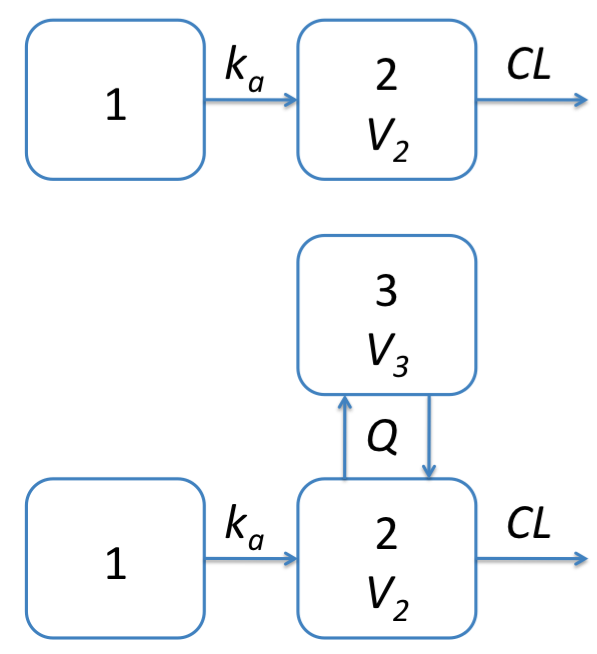
\includegraphics[width=1.5in]{./graphics/cptModels.png}
\caption{\label{one_two_cpt_models}One and two compartment models with first order absorption implemented in Torsten.}
\end{figure}

\subsection{Usage}
\label{sec:orgf3012f2}
\begin{minted}[breaklines=true,fontsize=\footnotesize,breakanywhere=true]{stan}
matrix = pmx_solve_onecpt(time, amt, rate, ii, evid, cmt, addl, ss, theta [, biovar, tlag ] )
\end{minted}

\subsection{Arguments}
\label{sec:org10352e3}
See Tables in Section \ref{sec:org02ca7f5}.
\subsection{Return value}
\label{sec:org649e9bd}
An \texttt{ncmt}-by-\texttt{nt} matrix, where \texttt{nt} is the number of time steps and \texttt{ncmt=2} is the number of compartments.
\subsection{Note}
\label{sec:org83e8503}
\begin{itemize}
\item ODE Parameters \texttt{theta} should consist of \(CL\), \(V_2\), \(k_a\), in that order.
\item \texttt{biovar} and \texttt{tlag} are optional, so that the following are allowed:
\end{itemize}
\begin{minted}[breaklines=true,fontsize=\footnotesize,breakanywhere=true]{stan}
pmx_solve_onecpt(..., theta);
pmx_solve_onecpt(..., theta, biovar);
pmx_solve_onecpt(..., theta, biovar, tlag);
\end{minted}
\begin{itemize}
\item Setting \(k_a = 0\) eliminates the first-order absorption.
\end{itemize}

\section{Two Compartment Model}
\label{sec:orgc2ace93}
\subsection{Description}
\label{sec:org8e248ad}
Function \texttt{pmx\_solve\_twocpt} solves a two-compartment PK
model (Figure \ref{one_two_cpt_models}). The model obtains the mass \((y_1, y_2, y_3)\) in each compartment
by solving the ODEs
\begin{align} \label{eq:twocpt}
  y_1' &= -k_a y_1 \\
  y_2' &= k_a y_1 - \left(\frac{CL}{V_2} + \frac{Q}{V_2}\right) y_2 +  \frac{Q}{V_3}  y_3  \\
  y_3' &= \frac{Q}{V_2} y_2 - \frac{Q}{V_3} y_3
\end{align}
The plasma concentrations of parent drug in the central compartment
can then be calculated as \(c=y_2/V_2\).

\subsection{Usage}
\label{sec:org38737c1}
\index{Two Compartment Model}
\begin{minted}[breaklines=true,fontsize=\footnotesize,breakanywhere=true]{stan}
matrix = pmx_solve_twocpt(time, amt, rate, ii, evid, cmt, addl, ss, theta [, biovar, tlag ] )
\end{minted}

\subsection{Arguments}
\label{sec:org3243539}
See Tables in Section \ref{sec:org02ca7f5}.
\subsection{Return value}
\label{sec:orgae1f71d}
An \texttt{ncmt}-by-\texttt{nt} matrix, where \texttt{nt} is the number of time steps and \texttt{ncmt=3} is the number of compartments.

\subsection{Note}
\label{sec:orgb724980}
\begin{itemize}
\item ODE Parameters \texttt{theta} consists of \(CL\), \(Q\), \(V_2\), \(V_3\), \(k_a\).
\item \texttt{biovar} and \texttt{tlag} are optional, so that the following are allowed:
\end{itemize}
\begin{minted}[breaklines=true,fontsize=\footnotesize,breakanywhere=true]{stan}
pmx_solve_twocpt(..., theta);
pmx_solve_twocpt(..., theta, biovar);
pmx_solve_twocpt(..., theta, biovar, tlag);
\end{minted}
\begin{itemize}
\item Setting \(k_a = 0\) eliminates the first-order absorption.
\end{itemize}

\section{General Linear ODE Model Function}
\label{sec:orgdba4f68}
\subsection{Description}
\label{sec:org56ce59e}
Function \texttt{pmx\_solve\_linode} solves a (piecewise) linear ODEs model with coefficients
in form of matrix \(K\)
\begin{equation}
y^\prime\left(t\right) = Ky\left(t\right)
\end{equation}
For example, in a two-compartment model with first order absorption, \(K\) is
\begin{equation}
  K = \left[\begin{array}{ccc}
              -k_a & 0 & 0 \\
              k_a & -\left(k_{10} + k_{12}\right) & k_{21} \\
              0 & k_{12} & -k_{21}
            \end{array}\right]
\end{equation}
where \(k_{10}=CL/V_2\), \(k_{12}=Q/V_2\), and \(k_{21}=Q/V_3\).

\subsection{Usage}
\label{sec:org24d89d8}
\index{General linear model}
\begin{minted}[breaklines=true,fontsize=\footnotesize,breakanywhere=true]{stan}
matrix = pmx_solve_linode(time, amt, rate, ii, evid, cmt, addl, ss, K, biovar, tlag )
\end{minted}

\subsection{Arguments}
\label{sec:org14ee903}
\begin{itemize}
\item \texttt{K}
System parameters. \texttt{K} can be either
\begin{itemize}
\item a \mintinline[breaklines=true,fontsize=\footnotesize,breakanywhere=true]{stan}{matrix} for constant parameters in all events, or
\item an array of matrices \mintinline[breaklines=true,fontsize=\footnotesize,breakanywhere=true]{stan}{matrix K[nt]} so that the \(i\)th entry of the array describes
the model parameters for time interval \((t_{i-1}, t_i)\),
and the number of the rows equals to the number of event time \texttt{nt}.
\end{itemize}
\item See Tables in Section \ref{sec:org02ca7f5} for the rest of arguments.
\end{itemize}
\subsection{Return value}
\label{sec:org5ab943c}
An \texttt{n}-by-\texttt{nt} matrix, where \texttt{nt} is the number of time steps and \texttt{n} is the number of rows(columns) of square matrix \texttt{K}.

\section{General ODE Model Function}
\label{sec:org337e56e}
\subsection{Description}
\label{sec:org63616ec}
Function \texttt{pmx\_solve\_adams}, \texttt{pmx\_solve\_bdf}, and \texttt{pmx\_solve\_rk45} solve a first-order ODE system
specified by user-specified right-hand-side function \texttt{ODE\_rhs} \(f\)
\begin{equation*}
y'(t) = f(t, y(t))
\end{equation*}
In the case where the \texttt{rate} vector \(r\) is non-zero, this equation becomes:
\begin{equation*}
y'(t) = f(t, y(t)) + r
\end{equation*}
\subsection{Usage}
\label{sec:orgdaea332}
\index{General ODE Model}
\begin{minted}[breaklines=true,fontsize=\footnotesize,breakanywhere=true]{stan}
matrix pmx_solve_[adams || rk45 || bdf](ODE_rhs, int nCmt, time, amt, rate, ii, evid, cmt, addl, ss, theta, [ biovar, tlag, real[,] x_r, int [,] x_i, real rel_tol, real abs_tol, int max_step, real as_rel_tol, real as_abs_tol, int as_max_step ] );
\end{minted}
Here \mintinline[breaklines=true,fontsize=\footnotesize,breakanywhere=true]{stan}{[adams || rk45 || bdf]} indicates the
function name can use any of the three suffixes. See below.

\subsection{Arguments}
\label{sec:org605fb37}
\begin{itemize}
\item \texttt{ODE\_rhs}
ODE right-hand-side \(f\). It should be defined in
\mintinline[breaklines=true,fontsize=\footnotesize,breakanywhere=true]{stan}{functions} block and has the following format
\end{itemize}
\begin{minted}[breaklines=true,fontsize=\footnotesize,breakanywhere=true]{stan}
vector = f(real t, vector y, array[] real param, array[] real dat_r, array[] int dat_i) {...}
\end{minted}
Here \texttt{t} is time, \texttt{y} the unknowns of ODE, \texttt{param} the parameters, \texttt{dat\textbackslash{}\_r} the real data, \texttt{dat\textbackslash{}\_i}
the integer data. \texttt{param},
\texttt{dat\textbackslash{}\_r}, and \texttt{dat\textbackslash{}\_i} are from
the entry of \texttt{theta}, \texttt{x\_r},
and \texttt{x\_i} corresponding to
\texttt{t}, respectively.
\(f\) should not include dosing rates in its
definition, as Torsten automatically update \(f\)
when the corresponding event indicates infusion dosage.
\begin{itemize}
\item \texttt{nCmt}
The number of compartments, equivalently, the dimension of the ODE system.
\item \texttt{x\_r}
2d arary real data to be passed to ODE RHS. If specified, its 1st
dimension should have the same size as \texttt{time}.
\item \texttt{x\_i}
2d arary integer data to be passed to ODE RHS. If specified, its 1st
dimension should have the same size as \texttt{time}.
\item \texttt{rel\_tol}
The relative tolerance for numerical integration, default to 1.0E-6.
\item \texttt{abs\_tol}
The absolute tolerance for numerical integration, default to 1.0E-6.
\item \texttt{max\_step}
The maximum number of steps in numerical integration, default to \(10^6\).
\item \texttt{as\_rel\_tol}
The relative tolerance for algebra solver for steady state solution, default to 1.0E-6.
\item \texttt{as\_abs\_tol}
The absolute tolerance for algebra solver for steady state solution, default to 1.0E-6.
\item \texttt{as\_max\_step}
The maximum number of interations in algebra solver for steady state solution, default to \(10^2\).
\item See Tables in Section \ref{sec:org02ca7f5} for the rest of arguments.
\end{itemize}

\subsection{Return value}
\label{sec:orgab3dea0}
An \texttt{nCmt}-by-\texttt{nt} matrix, where \texttt{nt} is the size of \texttt{time}.
\subsection{Note}
\label{sec:org58a342f}
\begin{itemize}
\item See Section \ref{sec:org2654f2a} for different types of integrator and general guidance.
\item See Section \ref{sec:org2654f2a} for comments on accuracy and tolerance.
\item The default values of \texttt{atol},
\texttt{rtol}, and \texttt{max\_step} are
based on a limited amount of PKPD test problems and should not be considered as
universally applicable. We strongly recommend user to set these values
according to physical intuition and numerical tests. See also Section \ref{sec:org2654f2a}.
\item With optional arguments indicated by square bracket, the following calls are allowed:
\end{itemize}
\begin{minted}[breaklines=true,fontsize=\footnotesize,breakanywhere=true]{stan}
pmx_solve_[adams || rk45 || bdf](..., theta);
pmx_solve_[adams || rk45 || bdf](..., theta, rel_tol, abs_tol, max_step);
pmx_solve_[adams || rk45 || bdf](..., theta, rel_tol, abs_tol, max_step, as_rel_tol, as_abs_tol, as_max_step);
pmx_solve_[adams || rk45 || bdf](..., theta, biovar);
pmx_solve_[adams || rk45 || bdf](..., theta, biovar, rel_tol, abs_tol, max_step);
pmx_solve_[adams || rk45 || bdf](..., theta, biovar, rel_tol, abs_tol, max_step, as_rel_tol, as_abs_tol, as_max_step);
pmx_solve_[adams || rk45 || bdf](..., theta, biovar, tlag);
pmx_solve_[adams || rk45 || bdf](..., theta, biovar, tlag, rel_tol, abs_tol, max_step);
pmx_solve_[adams || rk45 || bdf](..., theta, biovar, tlag, rel_tol, abs_tol, max_step, as_rel_tol, as_abs_tol, as_max_step);
pmx_solve_[adams || rk45 || bdf](..., theta, biovar, tlag, x_r);
pmx_solve_[adams || rk45 || bdf](..., theta, biovar, tlag, x_r, rel_tol, abs_tol, max_step);
pmx_solve_[adams || rk45 || bdf](..., theta, biovar, tlag, x_r, rel_tol, abs_tol, max_step, as_rel_tol, as_abs_tol, as_max_step);
pmx_solve_[adams || rk45 || bdf](..., theta, biovar, tlag, x_r, x_i);
pmx_solve_[adams || rk45 || bdf](..., theta, biovar, tlag, x_r, x_i, rel_tol, abs_tol, max_step);
pmx_solve_[adams || rk45 || bdf](..., theta, biovar, tlag, x_r, x_i, rel_tol, abs_tol, max_step, as_rel_tol, as_abs_tol, as_max_step);
\end{minted}

\section{PK-Effect Compartment Model Function}
\label{sec:org9ff6f70}
\index{PK effcpt Model}
\subsection{Description}
\label{sec:org997c5bb}
Indirect linking between PK and PD models can be realized by considering a hypothetical effect compartment. Function \texttt{pmx\_solve\_onecpt\_effcpt} solves the one-compartment model but with an additional compartment that is connected to the central compartment using a first-order rate parameter.
\begin{align}\label{eq:onecpt_effcpt}
  y_1' &= -k_a y_1, \\
  y_2' &= k_a y_1 - \left(\frac{CL}{V_2} + \frac{Q}{V_2}\right) y_2.
  y_e' &= k_e y_2 - k_ey_e.
\end{align}
Similarly, \texttt{pmx\_solve\_twocpt\_effcpt} solves the two-compartment model with an effect compartment.
\begin{align}\label{eq:onecpt_effcpt}
  y_1' &= -k_a y_1 \\
  y_2' &= k_a y_1 - \left(\frac{CL}{V_2} + \frac{Q}{V_2}\right) y_2 +  \frac{Q}{V_3}  y_3  \\
  y_3' &= \frac{Q}{V_2} y_2 - \frac{Q}{V_3} y_3
  y_e' &= k_e y_2 - k_ey_e.
\end{align}
\subsection{Usage}
\label{sec:orga2d9dc2}
\begin{minted}[breaklines=true,fontsize=\footnotesize,breakanywhere=true]{stan}
matrix pmx_solve_onecpt_effcpt(time, amt, rate, ii, evid, cmt, addl, ss, theta [, biovar, tlag ] );
matrix pmx_solve_twocpt_effcpt(time, amt, rate, ii, evid, cmt, addl, ss, theta [, biovar, tlag ] );
\end{minted}
\subsection{Arguments}
\label{sec:org3243540}
See Tables in Section \ref{sec:org02ca7f5}.
\subsection{Return value}
\label{sec:org84c1334}
An \texttt{ncmt}-by-\texttt{nt} matrix, where \texttt{nt} is the number of time steps and \texttt{ncmt} is the number of compartments, thus \texttt{ncmt=3} for \texttt{pmx\_solve\_onecpt\_effcpt} and \texttt{ncmt=4} for \texttt{pmx\_solve\_twocpt\_effcpt}.

\section{Coupled ODE Model Function}
\label{sec:org9ff6f77}
\index{coupled ODE Model}
\subsection{Description}
\label{sec:org997c5ba}
When the ODE system consists of two subsystems in form of
\begin{align*}
  y_1^\prime &= f_1(t, y_1), \\
  y_2^\prime &= f_2(t, y_1, y_2),
\end{align*}
with \(y_1\), \(y_2\), \(f_1\), and \(f_2\) being vector-valued functions, and
\(y_1^\prime\) independent of \(y_2\), the solution can be
accelerated if \(y_1\) admits an analytical solution which can
be introduced into the ODE for \(y_2\) for numerical
integration. This structure arises in PK/PD
models, where \(y_1\) describes a forcing PK function and \(y_2\) the PD
effects. In the example of a Friberg-Karlsson
semi-mechanistic model(see below), we observe an average speedup of
\(\sim 47 \pm 18 \%\) when using the mix solver in lieu of the numerical
integrator. In the context, currently the couple solver supports one-
\& two-compartment for PK model, and \texttt{rk45} \&
\texttt{bdf} integrator for nonlinear PD model.
\subsection{Usage}
\label{sec:orga2d9dc1}
\begin{minted}[breaklines=true,fontsize=\footnotesize,breakanywhere=true]{stan}
matrix pmx_solve_onecpt_[ rk45 || bdf ](reduced_ODE_system, int nOde, time, amt, rate, ii, evid, cmt, addl, ss, theta, biovar, tlag [, real rel_tol, real abs_tol, int max_step, real as_rel_tol, real as_abs_tol, int as_max_step ] );
matrix pmx_solve_twocpt_[ rk45 || bdf ](reduced_ODE_system, int nOde, time, amt, rate, ii, evid, cmt, addl, ss, theta, biovar, tlag [, real rel_tol, real abs_tol, int max_step, real as_rel_tol, real as_abs_tol, int as_max_step ] );
\end{minted}
\subsection{Arguments}
\label{sec:org1b037b1}
\begin{itemize}
\item \texttt{reduced\_ODE\_rhs}
The system  numerically solve (\(y_2\) in the above discussion, also called the
\emph{reduced system} and \texttt{nOde} the number of equations in
the \uline{reduced} system. The function that defines a reduced
system has an almost identical signature to that used for a full
system, but takes one additional argument: \(y_1\), the PK states,
i.e. solution to the PK ODEs.
\begin{minted}[breaklines=true,fontsize=\footnotesize,breakanywhere=true]{stan}
vector reduced_ODE_rhs(real t, vector y2, vector y1, array[] real theta, array[] real x_r, array[] int x_i)
\end{minted}
\item \texttt{nCmt}
The number of compartments. Equivalently, the dimension of the ODE system.
\item \texttt{rel\_tol}
The relative tolerance for numerical integration, default to 1.0E-6.
\item \texttt{abs\_tol}
The absolute tolerance for numerical integration, default to 1.0E-6.
\item \texttt{max\_step}
The maximum number of steps in numerical integration, default to \(10^6\).
\item See Tables in Section \ref{sec:org02ca7f5} for the rest of arguments.
\end{itemize}
\subsection{Return value}
\label{sec:org84c1333}
An \texttt{(nPk + nOde)} \texttimes{} \texttt{nt} matrix, where \texttt{nt} is the size of
\texttt{time}, and \texttt{nPk} equals to 2 in
\texttt{pmx\_solve\_onecpt\_} functions
and 3 in \texttt{pmx\_solve\_twocpt\_} functions.

\section{General ODE-based Population Model Function}
\label{sec:org6157bc2}
\subsection{Description}
\label{sec:org208bcf5}
All the preivous functions solves for a single sunject. Torsten also
provides population modeling counterparts for ODE solutions. The
functions solve for a population that share an ODE model but with
subject-level parameters and event specifications and have similar
signatures to single-subject functions, except that now events
arguments \texttt{time}, \texttt{amt}, \texttt{rate}, \texttt{ii},
\texttt{evid}, \texttt{cmt},
\texttt{addl}, \texttt{ss} specifies the entire
population, one subject after another.
\subsection{Usage}
\label{sec:orgca1a777}
\index{General ODE Model}
\begin{minted}[breaklines=true,fontsize=\footnotesize,breakanywhere=true]{stan}
matrix pmx_solve_group_[adams || rk45 || bdf](ODE_rhs, int nCmt, array[] int len, time, amt, rate, ii, evid, cmt, addl, ss, theta, [ biovar, tlag, real[,] x_r, int [,] x_i, real rel_tol, real abs_tol, int max_step, real as_rel_tol, real as_abs_tol, int as_max_step ] );
\end{minted}
Here \mintinline[breaklines=true,fontsize=\footnotesize,breakanywhere=true]{stan}{[adams || rk45 || bdf]} indicates the
function name can be of any of the three suffixes. See Section \ref{sec:org2654f2a}.
\subsection{Arguments}
\label{sec:org8761582}
\begin{itemize}
\item \texttt{ODE\_rhs}
Same as in Section \ref{sec:org2654f2a}.
\item \texttt{time}, \texttt{amt}, \texttt{rate}, \texttt{ii}, \texttt{evid}, \texttt{cmt}, \texttt{addl}, \texttt{ss}
2d-array arguments that describe data record for the
entire population (see also Tables in Section \ref{sec:org02ca7f5}). They must have same size in the first
dimension. Take \texttt{evid} for example. Let \(N\) be the
population size, then \texttt{evid[1,]} to
\texttt{evid[n1,]} specifies events ID for subject 1,
\texttt{evid[n1 + 1,]} to
\texttt{evid[n1 + n2,]} for subject 2, etc. With \(n_i\)
being the number of events for subject \(i\), \(i=1, 2, \dots, N\), the
size of \texttt{evid}'s first dimension is \(\sum_{i}n_i\).
\item \texttt{len}
The length of data for each subject within
the above events arrays. The size of \texttt{len} equals
to population size \(N\).
\item \texttt{nCmt}
The number of compartments. Equivalently, the dimension of the ODE system.
\item \texttt{x\_r}
2d arary real data to be passed to ODE RHS. If specified, its 1st
dimension should have the same size as \texttt{time}.
\item \texttt{x\_i}
2d arary integer data to be passed to ODE RHS. If specified, its 1st
dimension should have the same size as \texttt{time}.
\item \texttt{rel\_tol}
The relative tolerance for numerical integration, default to 1.0E-6.
\item \texttt{abs\_tol}
The absolute tolerance for numerical integration, default to 1.0E-6.
\item \texttt{max\_step}
The maximum number of steps in numerical integration, default to \(10^6\).
\item \texttt{as\_rel\_tol}
The relative tolerance for algebra solver for steady state solution, default to 1.0E-6.
\item \texttt{as\_abs\_tol}
The absolute tolerance for algebra solver for steady state solution, default to 1.0E-6.
\item \texttt{as\_max\_step}
The maximum number of interations in algebra solver for steady state solution, default to \(10^2\).
\end{itemize}
\subsection{Return value}
\label{sec:org0635278}
An \texttt{nCmt}-by-\texttt{nt} matrix, where \texttt{nt} is the total size of
events \(\sum_{i}n_i\).
\subsection{Note}
\label{sec:ode_pop_note}
\begin{itemize}
\item Similar to single-subject solvers, three numerical integrator are provided:
\begin{itemize}
\item \texttt{pmx\_solve\_group\_adams}: Adams-Moulton method,
\item \texttt{pmx\_solve\_group\_bdf}: Backward-differentiation formular,
\item \texttt{pmx\_solve\_group\_rk45}: Runge-Kutta 4/5 method.
\end{itemize}
\item With optional arguments indicated by square bracket, the following calls are allowed:
\end{itemize}
\begin{minted}[breaklines=true,fontsize=\footnotesize,breakanywhere=true]{stan}
pmx_solve_group_[adams || rk45 || bdf](..., theta);
pmx_solve_group_[adams || rk45 || bdf](..., theta, rel_tol, abs_tol, max_step);
pmx_solve_group_[adams || rk45 || bdf](..., theta, rel_tol, abs_tol, max_step, as_rel_tol, as_abs_tol, as_max_step);
pmx_solve_group_[adams || rk45 || bdf](..., theta, biovar);
pmx_solve_group_[adams || rk45 || bdf](..., theta, biovar, rel_tol, abs_tol, max_step);
pmx_solve_group_[adams || rk45 || bdf](..., theta, biovar, rel_tol, abs_tol, max_step, as_rel_tol, as_abs_tol, as_max_step);
pmx_solve_group_[adams || rk45 || bdf](..., theta, biovar, tlag);
pmx_solve_group_[adams || rk45 || bdf](..., theta, biovar, tlag, rel_tol, abs_tol, max_step);
pmx_solve_group_[adams || rk45 || bdf](..., theta, biovar, tlag, rel_tol, abs_tol, max_step, as_rel_tol, as_abs_tol, as_max_step);
pmx_solve_group_[adams || rk45 || bdf](..., theta, biovar, tlag, x_r);
pmx_solve_group_[adams || rk45 || bdf](..., theta, biovar, tlag, x_r, rel_tol, abs_tol, max_step);
pmx_solve_group_[adams || rk45 || bdf](..., theta, biovar, tlag, x_r, rel_tol, abs_tol, max_step, as_rel_tol, as_abs_tol, as_max_step);
pmx_solve_group_[adams || rk45 || bdf](..., theta, biovar, tlag, x_r, x_i);
pmx_solve_group_[adams || rk45 || bdf](..., theta, biovar, tlag, x_r, x_i, rel_tol, abs_tol, max_step);
pmx_solve_group_[adams || rk45 || bdf](..., theta, biovar, tlag, x_r, x_i, rel_tol, abs_tol, max_step, as_rel_tol, as_abs_tol, as_max_step);
\end{minted}
\begin{itemize}
\item The group solvers support paralleisation through Message Passing
Interface(MPI). One can access this feature through \texttt{cmdstan} or
\texttt{cmdstanr} interface.
\end{itemize}
\begin{minted}[breaklines=true,fontsize=\footnotesize,breakanywhere=true]{bash}
# cmdstan interface user need to add "TORSTEN_MPI=1" and
# "TBB_CXX_TYPE=gcc" in "cmdstan/make/local" file. In linux & macos
# this can be done as
echo "TORSTEN_MPI=1" > cmdstan/make/local
echo "TBB_CXX_TYPE=gcc" > cmdstan/make/local # "gcc" should be replaced by user's C compiler
make path-to-model/model_name
mpiexec -n number_of_processes model_name sample... # additional cmdstan options
\end{minted}
\begin{minted}[breaklines=true,fontsize=\footnotesize,breakanywhere=true]{r}
library("cmdstanr")
cmdstan_make_local(cpp_options = list("TORSTEN_MPI" = "1", "TBB_CXX_TYPE"="gcc"))  # "gcc" should be replaced by user's C compiler
rebuild_cmdstan()
mod <- cmdstan_model(path-to-model-file, quiet=FALSE, force_recompile=TRUE)
f <- mod$sample_mpi(data = ..., chains = 1, mpi_args = list("n" = number_of_processes), refresh = 200)
\end{minted}
Here \(n\) denotes number of MPI processes, so that \(N\)
ODE systems (each specified by a same RHS function and
subject-dependent events) are distributed to and solved by \(n\)
processes evenly. Note that to access this feature user must have
MPI installed, and some MPI installation may require set additional
compiler arguments, such as \texttt{CXXLFAGS} and \texttt{LDFLAGS}.

\section{ODE  integrator function}
\label{sec:org2654f2a}
\subsection{Description}
\label{sec:orge3aae27}
Torsten provides its own implementation of ODE solvers that solves
\begin{equation*}
  y'(t) = f(t, y(t)), \quad y(t_0) = y_0
\end{equation*}
for \(y\). These solvers
are customized for Torsten applications and different from those found
in Stan. The general ODE PMX solvers in previous sections are internally powered
by these functions.
\subsection{Usage}
\label{sec:org13cb90b}
\index{PMX ODE integrators}
\begin{minted}[breaklines=true,fontsize=\footnotesize,breakanywhere=true]{stan}
array[] vector pmx_ode_[ adams || bdf || rk45 || ckrk ](ODE_rhs, vector y0, real t0, array[] real ts, ...);
array[] vector pmx_ode_[ adams || bdf || rk45 || ckrk ]_ctrl(ODE_rhs, vector y0, real t0, array[] real ts, real rtol, real atol, int max_step, ...);
\end{minted}
\subsection{Arguments}
\label{sec:orgcf984ad}
\begin{itemize}
\item \texttt{ODE\_rhs}
Function that specifies the right-hand-side \(f\).
It should be defined in
\mintinline[breaklines=true,fontsize=\footnotesize,breakanywhere=true]{stan}{functions} block and has the following format
\end{itemize}
\begin{minted}[breaklines=true,fontsize=\footnotesize,breakanywhere=true]{stan}
vector = f(real t, vector y, ...) {}
\end{minted}
Here \texttt{t} is time, \texttt{y} the unknowns of ODE, \texttt{...} the arbitrary number number (and type) of parameters.
\begin{itemize}
\item \texttt{y0}
Initial condition \(y_0\).
\item \texttt{t0}
Initial time \(t_0\).
\item \texttt{ts}
Output time when solution is seeked.
\item \texttt{...}
Parameters to be passed to \texttt{ODE\_rhs} function.
\item \texttt{rtol}
Relative tolerance, default to 1.e-6(\texttt{rk45}) and 1.e-8(\texttt{adams} and \texttt{bdf}).
\item \texttt{atol}
Absolute tolerance, default to 1.e-6(\texttt{rk45}) and 1.e-8(\texttt{adams} and \texttt{bdf}).
\item \texttt{max\_step}
Maximum number of steps allowed between neighboring time in \texttt{ts},
default to 100000.
\end{itemize}
\subsection{Return value}
\label{sec:org0bffd09}
A \texttt{n}-array of \texttt{nd}-vectors, where \texttt{n} is the size of \texttt{ts}
and \texttt{nd} the dimension of the system.
\subsection{Note}
\label{sec:orgf701db1}
\begin{itemize}
\item Four numerical integrator are provided:
\begin{itemize}
\item \texttt{pmx\_ode\_adams}: Adams-Moulton method,
\item \texttt{pmx\_ode\_bdf}: Backward-differentiation formular,
\item \texttt{pmx\_ode\_rk45}: Runge-Kutta 4/5 method.
\item \texttt{pmx\_ode\_ckrk}: Cash-Karp 4/5 method.
\end{itemize}
When not equipped with further understanding of the ODE system, as a
rule of thumb we suggest user try
\texttt{rk45} integrator first, \texttt{bdf}
integrator when the system is suspected to be stiff, and
\texttt{adams} and \texttt{ckrk} when a non-stiff system needs to be solved
with higher accuracy/smaller tolerance, or long integration time.

\item All four integrators support adaptive stepping. To achieve
that, at step \(i\) estimated error \(e_i\) is calculated and
compared with given tolerance so that
\begin{equation}
  e_i < \Vert\text{rtol} \times \tilde{y} + \text{atol}\Vert
\end{equation}
Here \(\tilde{y}\) is the numerical solution of \(y\) at current
step and \(\Vert \cdot \Vert\) indicates certain norm. When the above check fails, the solver attempts
to reduce step size and retry. The default values of \texttt{atol},
\texttt{rtol}, and \texttt{max\_step} are
based on Stan's ODE functions and should not be considered as
optimal. User should make problem-dependent
decision on \texttt{rtol} and \texttt{atol},
according to estimated scale of the unknowns, so that the error
would not affect inference on statistical variance of quantities
that enter the Stan model. In particular, when an unknown can be neglected
below certain threshold without affecting the rest of
the dynamic system, setting
\texttt{atol} greater than that threshold will avoid
spurious and error-prone computation. See
\cite{hindmarsh_cvodes_2020} and
1.4 of \cite{shampine_solving_2003} for details.

\end{itemize}

\section{Univariate integral}
\label{sec:org5024381}
\index{univariate integral}
\begin{minted}[breaklines=true,fontsize=\footnotesize,breakanywhere=true]{stan}
real univariate_integral_rk45(f, t0, t1, theta, x_r, x_i)
\end{minted}
\begin{minted}[breaklines=true,fontsize=\footnotesize,breakanywhere=true]{stan}
real univariate_integral_bdf(f, t0, t1, theta, x_r, x_i)
\end{minted}
Based on the ODE solver capability in Stan, Torsten provides functions
calculating the integral of a univariate function. The integrand function \(f\) must follow the signature
\begin{minted}[breaklines=true,fontsize=\footnotesize,breakanywhere=true]{stan}
  real f(real t, array[] real theta, array[] real x_r, array[] int x_i) {
    /* ... */
}
\end{minted}

\section{Piecewise linear interpolation}
\label{sec:org5f1a4b1}
\index{linear interpolation}
\begin{minted}[breaklines=true,fontsize=\footnotesize,breakanywhere=true]{stan}
real linear_interpolation(real xout, array[] real x, array[] real y)
\end{minted}
\begin{minted}[breaklines=true,fontsize=\footnotesize,breakanywhere=true]{stan}
array[] real linear_interpolation(array[] real xout, array[] real x, array[] real y)
\end{minted}
Torsten also provides function \texttt{linear\_interpolation} for piecewise linear interpolation over a
set of x, y pairs. It returns the values of a piecewise linear
function at specified values \texttt{xout} of the first function argument. The
function is specified in terms of a set of x, y
pairs. Specifically, \texttt{linear\_interpolation} implements the following function
\begin{align*}
  y_{\text{out}} = \left\{\begin{array}{ll}
                 y_1, & x_{\text{out}} < x_1 \\
                 y_i + \frac{y_{i+1} - y_i}{x_{i+1} - x_i}
                 \left(x_{\text{out}} - x_i\right), & x_{\text{out}} \in [x_i, x_{i+1}) \\
                 y_n, & x_{\text{out}} \ge x_n
                          \end{array}\right.
\end{align*}
\begin{itemize}
\item The x values must be in increasing order, i.e. \(x_i < x_{i+1}\).
\item All three arguments may be data or parameters.
\end{itemize}

\chapter{Examples}
\label{sec:org5ad4b3a}
All the PMX models in this chapter can be found in
\texttt{Torsten/example-models} directory:
\begin{itemize}
\item \href{https://github.com/metrumresearchgroup/Torsten/tree/master/example-models/pk2cpt}{Two-compartment model}
\item \href{https://github.com/metrumresearchgroup/Torsten/tree/master/example-models/pk2cpt\_linode}{Two-compartment model by linear ODEs}
\item \href{https://github.com/metrumresearchgroup/Torsten/tree/master/example-models/pk2cpt\_ode}{two-compartment model by numerical ODEs}
\item \href{https://github.com/metrumresearchgroup/Torsten/tree/master/example-models/FK\_coupled}{Joint PK/PD model}
\item \href{https://github.com/metrumresearchgroup/Torsten/tree/master/example-models/twocpt\_population}{Two-compartment popPK model}
\item \href{https://github.com/metrumresearchgroup/Torsten/tree/master/example-models/lotka\_volterra\_ode\_group\_model}{Group of ODEs}
\item \href{https://github.com/metrumresearchgroup/Torsten/tree/master/example-models/effCpt}{Effective compartment model}
\item \href{https://github.com/metrumresearchgroup/Torsten/tree/master/example-models/FribergKarlsson}{PopPKPD model}
\end{itemize}

\section{Two-compartment model for single patient}
\label{sec:org4b8e202}
We model drug absorption in a single patient and simulate plasma drug concentrations:

\begin{itemize}
\item Multiple Doses: 1250 mg, every 12 hours, for a total of 15 doses
\item PK measured at 0.083, 0.167, 0.25, 0.5, 0.75, 1, 1.5, 2, 4, 6,
8, 10 and 12 hours after 1st, 2nd, and 15th dose. In addition, the
PK is measured every 12 hours throughout the trial.
\end{itemize}

With the plasma concentration \(\hat{c}\) using
\ref{sec:orgc2ace93}, we simulate \(c\) according to:
\begin{align*}
  \log\left(c\right) &\sim N\left(\log\left(\widehat{c}\right),\sigma^2\right) \\
  \left(CL, Q, V_2, V_3, ka\right) &= \left(5\ {\rm L/h}, 8\  {\rm L/h}, 20\  {\rm L},  70\ {\rm L}, 1.2\ {\rm h^{-1}} \right) \\
  \sigma^2 &= 0.01
\end{align*}
The data are generated using the R package \texttt{mrgsolve} \cite{Baron000}.

Code below shows how Torsten function \texttt{pmx\_solve\_twocpt} can be used to fit the above model.

\begin{minted}[breaklines=true,fontsize=\footnotesize,breakanywhere=true]{stan}
data{
  int<lower = 1> nt;  // number of events
  int<lower = 1> nObs;  // number of observation
  int<lower = 1> iObs[nObs];  // index of observation

  // NONMEM data
  int<lower = 1> cmt[nt];
  int evid[nt];
  int addl[nt];
  int ss[nt];
  real amt[nt];
  real time[nt];
  real rate[nt];
  real ii[nt];

  vector<lower = 0>[nObs] cObs;  // observed concentration (Dependent Variable)
}

transformed data{
  vector[nObs] logCObs = log(cObs);
  int nTheta = 5;  // number of ODE parameters in Two Compartment Model
  int nCmt = 3;  // number of compartments in model
}

parameters{
  real<lower = 0> CL;
  real<lower = 0> Q;
  real<lower = 0> V1;
  real<lower = 0> V2;
  real<lower = 0> ka;
  real<lower = 0> sigma;
}

transformed parameters{
  real theta[nTheta];  // ODE parameters
  row_vector<lower = 0>[nt] cHat;
  vector<lower = 0>[nObs] cHatObs;
  matrix<lower = 0>[nCmt, nt] x;

  theta[1] = CL;
  theta[2] = Q;
  theta[3] = V1;
  theta[4] = V2;
  theta[5] = ka;

  x = pmx_solve_twocpt(time, amt, rate, ii, evid, cmt, addl, ss, theta);

  cHat = x[2, :] ./ V1; // we're interested in the amount in the second compartment

  cHatObs = cHat'[iObs]; // predictions for observed data recors
}

model{
  // informative prior
  CL ~ lognormal(log(10), 0.25);
  Q ~ lognormal(log(15), 0.5);
  V1 ~ lognormal(log(35), 0.25);
  V2 ~ lognormal(log(105), 0.5);
  ka ~ lognormal(log(2.5), 1);
  sigma ~ cauchy(0, 1);

  logCObs ~ normal(log(cHatObs), sigma);
}
\end{minted}

Four MCMC chains of 2000 iterations (1000 warmup iterations and 1000
sampling iterations) are simulated. 1000 samples per chain were used for the subsequent analyses.
The MCMC history plots(Figure \ref{twocpt_mcmc_history})
suggest that the 4 chains have converged to common distributions for
all of the key model parameters. The fit to the plasma concentration
data (Figure \ref{twocpt_mcmc_predict}) are in close agreement with the
data, which is not surprising since the fitted model is identical to
the one used to simulate the data. Similarly the parameter posterior
density can be examined in Figure \ref{twocpt_mcmc_posterior} and shows
consistency with the values used for simulation. Another way to
summarize the posterior is through \texttt{cmdstanr}'s \texttt{summary} method.

\begin{minted}[breaklines=true,fontsize=\footnotesize,breakanywhere=true]{r}
## fit is a CmdStanMCMC object returned by sampling. See cmdstanr reference.
> pars = c("CL", "Q", "V1", "V2", "ka", "sigma")
> fit$summary(pars)
# A tibble: 6 x 10
  variable   mean median     sd    mad      q5    q95  rhat ess_bulk ess_tail
  <chr>     <dbl>  <dbl>  <dbl>  <dbl>   <dbl>  <dbl> <dbl>    <dbl>    <dbl>
1 CL        4.82   4.83  0.0910 0.0870  4.68    4.97   1.00    1439.    1067.
2 Q         7.56   7.55  0.588  0.586   6.61    8.56   1.00    1256.    1235.
3 V1       21.1   21.1   2.50   2.45   17.1    25.3    1.00    1057.    1177.
4 V2       76.1   76.1   5.33   4.93   67.5    84.9    1.01    1585.    1372.
5 ka        1.23   1.23  0.175  0.174   0.958   1.52   1.00    1070.    1122.
6 sigma     0.109  0.108 0.0117 0.0111  0.0911  0.130  1.01    1414.     905.
\end{minted}

\begin{figure}[htbp]
\centering
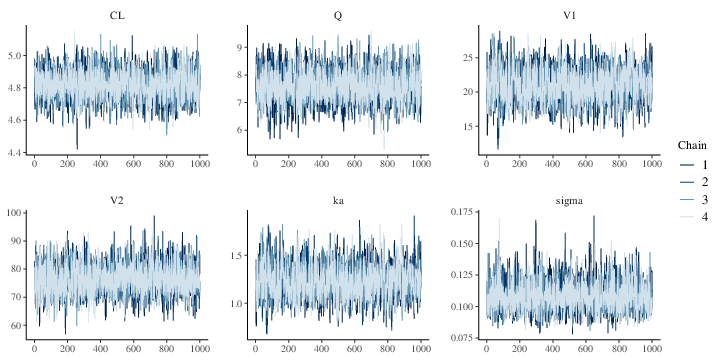
\includegraphics[width=\linewidth]{../example-models/pk2cpt/deliv/figure/history.pdf}
\caption{\label{twocpt_mcmc_history}MCMC history plots for the parameters of a two compartment model with first order absorption (each color corresponds to a different chain)}
\end{figure}

\begin{figure}[htbp]
\centering
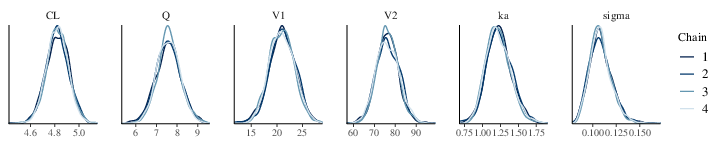
\includegraphics[width=\linewidth]{../example-models/pk2cpt/deliv/figure/density.pdf}
\caption{\label{twocpt_mcmc_posterior}Posterior marginal densities of the Model Parameters of a two compartment model with first order absorption (each color corresponds to a different chain)}
\end{figure}

\begin{figure}[htbp]
\centering
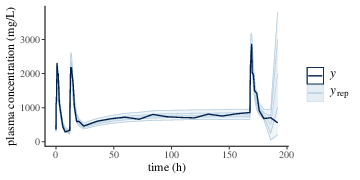
\includegraphics[width=0.5\linewidth]{../example-models/pk2cpt/deliv/figure/ppc_ribbon.pdf}
\caption{\label{twocpt_mcmc_predict}Predicted (\(y_{\text{rep}}\)) and observed (\(y\)) plasma drug concentrations of a two compartment model with first order absorption. \(y_{\text{rep}}\) is shown with posterior median, 50\%, 90\% credible intervals.}
\end{figure}

\section{Two-compartment model as a linear ODE model for single patient}
\label{sec:org12943da}
Using \texttt{pmx\_solve\_linode}, the following example fits a two-compartment model
with first order absorption. We omit \mintinline[breaklines=true,fontsize=\footnotesize,breakanywhere=true]{stan}{data} and
\mintinline[breaklines=true,fontsize=\footnotesize,breakanywhere=true]{stan}{model} block as they are identical to \ref{sec:org4b8e202} Example.

\begin{minted}[breaklines=true,fontsize=\footnotesize,breakanywhere=true]{stan}
transformed data{
  row_vector[nObs] logCObs = log(cObs);
  int nCmt = 3;
  real biovar[nCmt];
  real tlag[nCmt];

  for (i in 1:nCmt) {
    biovar[i] = 1;
    tlag[i] = 0;
  }
}

parameters{
  real<lower = 0> CL;
  real<lower = 0> Q;
  real<lower = 0> V1;
  real<lower = 0> V2;
  real<lower = 0> ka;
  real<lower = 0> sigma;
}

transformed parameters{
  matrix[3, 3] K;
  real k10 = CL / V1;
  real k12 = Q / V1;
  real k21 = Q / V2;
  row_vector<lower = 0>[nt] cHat;
  row_vector<lower = 0>[nObs] cHatObs;
  matrix<lower = 0>[3, nt] x;

  K = rep_matrix(0, 3, 3);

  K[1, 1] = -ka;
  K[2, 1] = ka;
  K[2, 2] = -(k10 + k12);
  K[2, 3] = k21;
  K[3, 2] = k12;
  K[3, 3] = -k21;

  x = pmx_solve_linode(time, amt, rate, ii, evid, cmt, addl, ss, K, biovar, tlag);

  cHat = row(x, 2) ./ V1;

  for(i in 1:nObs){
    cHatObs[i] = cHat[iObs[i]];  // predictions for observed data records
  }
}
\end{minted}

\section{Two-compartment model solved by numerical integrator for single patient}
\label{sec:org1ae9370}
Using \texttt{pmx\_solve\_rk45}, the following example fits a two-compartment model
with first order absorption. User-defined function
\texttt{ode\_rhs} describes the RHS of the ODEs.
\begin{minted}[breaklines=true,fontsize=\footnotesize,breakanywhere=true]{stan}
functions{
  vector ode_rhs(real t, vector x, array[] real parms, array[] real x_r, array[] int x_i){
    real CL = parms[1];
    real Q = parms[2];
    real V1 = parms[3];
    real V2 = parms[4];
    real ka = parms[5];

    real k10 = CL / V1;
    real k12 = Q / V1;
    real k21 = Q / V2;

    vector[3] y;

    y[1] = -ka*x[1];
    y[2] = ka*x[1] - (k10 + k12)*x[2] + k21*x[3];
    y[3] = k12*x[2] - k21*x[3];

    return y;
  }
}
\end{minted}

We omit \mintinline[breaklines=true,fontsize=\footnotesize,breakanywhere=true]{stan}{data} and
\mintinline[breaklines=true,fontsize=\footnotesize,breakanywhere=true]{stan}{model} block as they are identical to \ref{sec:org4b8e202} Example.

\begin{minted}[breaklines=true,fontsize=\footnotesize,breakanywhere=true]{stan}
transformed data {
  row_vector[nObs] logCObs = log(cObs);
  int nTheta = 5;   // number of parameters
  int nCmt = 3;   // number of compartments
}

parameters {
  real<lower = 0> CL;
  real<lower = 0> Q;
  real<lower = 0> V1;
  real<lower = 0> V2;
  real<lower = 0> ka;
  real<lower = 0> sigma;
}

transformed parameters {
  real theta[nTheta];
  row_vector<lower = 0>[nt] cHat;
  row_vector<lower = 0>[nObs] cHatObs;
  matrix<lower = 0>[3, nt] x;

  theta[1] = CL;
  theta[2] = Q;
  theta[3] = V1;
  theta[4] = V2;
  theta[5] = ka;

  x = pmx_solve_rk45(ode_rhs, 3, time, amt, rate, ii, evid, cmt, addl, ss, theta, 1e-5, 1e-8, 1e5);

  cHat = x[2, ] ./ V1;

  for(i in 1:nObs){
    cHatObs[i] = cHat[iObs[i]];  // predictions for observed data records
  }
}

model{
\end{minted}

\section{Joint PK-PD model}
\label{sec:fk_model}
\index{Friberg-Karlsson Model}
Neutropenia is observed in patients receiving an ME-2 drug. Our goal
is to model the relation between neutrophil counts and drug
exposure. As shown in Figure \ref{fig:FK_model}, the Friberg-Karlsson Semi-Mechanistic model \cite{friberg_mechanistic_2003} couples
a PK model with a PD
effect to describe a delayed feedback mechanism that keeps the
absolute neutrophil count (ANC) at the
baseline in a circulatory compartment (Circ), and
the drug's effect in
reducing the proliferation rate (prol).
The delay between prol and Circ is modeled using \(n\) transit
comparments with mean transit time MTT = \((n + 1)/k_{\text{tr}}\),
with \(k_{\text{tr}}\) the transit rate constant. In the current
example, we use the \ref{sec:orgc2ace93} for
PK model, and set \(n = 3\).

\begin{align}
  \log(\text{ANC})& \sim N(\log(y_{\text{circ}}), \sigma^2_{\text{ANC}}),  \\
  y_{\text{circ}}& = f_{\text{FK}}(\text{MTT}, \text{Circ}_{0}, \alpha, \gamma, c),
\end{align}
  where \(c\) is the drug concentration calculated from the PK model, and function \(f_{\text{FK}}\) represents solving the following
nonlinear ODE for \(y_{\text{circ}}\)
\begin{align}\label{eq:FK}
  \frac{dy_\mathrm{prol}}{dt} &= k_\mathrm{prol} y_\mathrm{prol} (1 - E_\mathrm{drug})\left(\frac{\text{Circ}_0}{y_\mathrm{circ}}\right)^\gamma - k_\mathrm{tr}y_\mathrm{prol}, \\
  \frac{dy_\mathrm{trans1}}{dt} &= k_\mathrm{tr} y_\mathrm{prol} - k_\mathrm{tr} y_\mathrm{trans1}, \\
  \frac{dy_\mathrm{trans2}}{dt} &= k_\mathrm{tr} y_\mathrm{trans1} - k_\mathrm{tr} y_\mathrm{trans2},  \\
  \frac{dy_\mathrm{trans3}}{dt} &= k_\mathrm{tr} y_\mathrm{trans2} - k_\mathrm{tr} y_\mathrm{trans3},  \\
  \frac{dy_\mathrm{circ}}{dt} &= k_\mathrm{tr} y_\mathrm{trans3} - k_\mathrm{tr} y_\mathrm{circ},
\end{align}
We use \(E_{\text{drug}} = \alpha c\) to model the linear effect of drug
concentration in central compartment, with
\(c=y_{\text{cent}}/V_{\text{cent}}\) based on PK solutions.

Since the ODEs specifying the Two Compartment Model
(Equation \eqref{eq:twocpt}) do not depend on the PD ODEs
(Equation \eqref{eq:FK}) and can be solved analytically
using Torsten's \mintinline[breaklines=true,fontsize=\footnotesize,breakanywhere=true]{stan}{pmx_solve_twocpt} function
we can specify solve the system using a coupled solver function. We do not
expect our system to be stiff and use the Runge-Kutta 4th/5th order
integrator.

\begin{figure}[htbp]
\centering
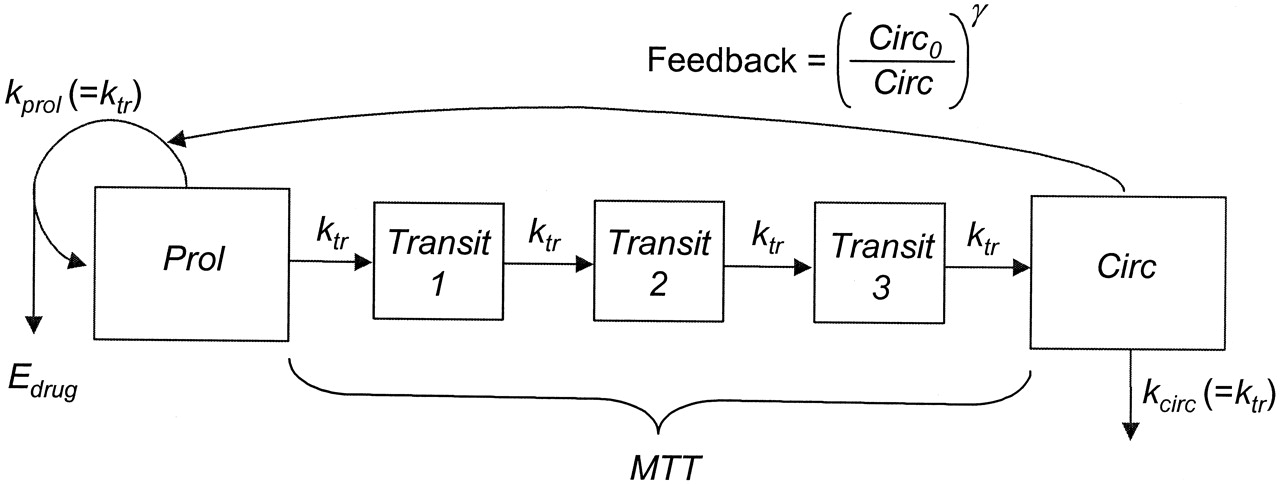
\includegraphics[width=0.8\textwidth]{./graphics/neutrophilModel.jpg}
\caption{\label{fig:FK_model}Friberg-Karlsson semi-mechanistic Model.}
\end{figure}


The model fitting is based on simulated data
\begin{align*}
  (\text{MTT}, \text{Circ}_{0}, \alpha, \gamma, k_{\text{tr}})& = (125, 5.0, 3 \times 10^{-4}, 0.17) \\
  \sigma^2_{\text{ANC}}& = 0.001.
\end{align*}

\begin{minted}[breaklines=true,fontsize=\footnotesize,breakanywhere=true]{stan}
functions{
  vector FK_ODE(real t, vector y, vector y_pk, array[] real theta, array[] real rdummy, array[] int idummy){
    /* PK variables */
    real VC = theta[3];

    /* PD variable */
    real mtt      = theta[6];
    real circ0    = theta[7];
    real alpha    = theta[8];
    real gamma    = theta[9];
    real ktr      = 4.0 / mtt;
    real prol     = y[1] + circ0;
    real transit1 = y[2] + circ0;
    real transit2 = y[3] + circ0;
    real transit3 = y[4] + circ0;
    real circ     = fmax(machine_precision(), y[5] + circ0);
    real conc     = y_pk[2] / VC;
    real EDrug    = alpha * conc;

    vector[5] dydt;

    dydt[1] = ktr * prol * ((1 - EDrug) * ((circ0 / circ)^gamma) - 1);
    dydt[2] = ktr * (prol - transit1);
    dydt[3] = ktr * (transit1 - transit2);
    dydt[4] = ktr * (transit2 - transit3);
    dydt[5] = ktr * (transit3 - circ);

    return dydt;
  }
}

data{
  int<lower = 1> nt;
  int<lower = 1> nObsPK;
  int<lower = 1> nObsPD;
  int<lower = 1> iObsPK[nObsPK];
  int<lower = 1> iObsPD[nObsPD];
  real<lower = 0> amt[nt];
  int<lower = 1> cmt[nt];
  int<lower = 0> evid[nt];
  real<lower = 0> time[nt];
  real<lower = 0> ii[nt];
  int<lower = 0> addl[nt];
  int<lower = 0> ss[nt];
  real rate[nt];
  vector<lower = 0>[nObsPK] cObs;
  vector<lower = 0>[nObsPD] neutObs;

  real<lower = 0> circ0Prior;
  real<lower = 0> circ0PriorCV;
  real<lower = 0> mttPrior;
  real<lower = 0> mttPriorCV;
  real<lower = 0> gammaPrior;
  real<lower = 0> gammaPriorCV;
  real<lower = 0> alphaPrior;
  real<lower = 0> alphaPriorCV;
}

transformed data{
  int nOde = 5;
  vector[nObsPK] logCObs;
  vector[nObsPD] logNeutObs;

  int nTheta = 9; // number of parameters
  int nIIV = 7; // parameters with IIV

  int n = 8;                        /* ODE dimension */
  real rtol = 1e-8;
  real atol = 1e-8;;
  int max_step = 100000;

  logCObs = log(cObs);
  logNeutObs = log(neutObs);
}

parameters{

  real<lower = 0> CL;
  real<lower = 0> Q;
  real<lower = 0> VC;
  real<lower = 0> VP;
  real<lower = 0> ka;
  real<lower = 0> mtt;
  real<lower = 0> circ0;
  real<lower = 0> alpha;
  real<lower = 0> gamma;
  real<lower = 0> sigma;
  real<lower = 0> sigmaNeut;

  // IIV parameters
  cholesky_factor_corr[nIIV] L;
  vector<lower = 0>[nIIV] omega;
}

transformed parameters{
  row_vector[nt] cHat;
  vector<lower = 0>[nObsPK] cHatObs;
  row_vector[nt] neutHat;
  vector<lower = 0>[nObsPD] neutHatObs;
  real<lower = 0> theta[nTheta];
  matrix[nOde + 3, nt] x;
  real biovar[nTheta] = rep_array(1.0, nTheta);
  real tlag[nTheta] = rep_array(0.0, nTheta);

  theta[1] = CL;
  theta[2] = Q;
  theta[3] = VC;
  theta[4] = VP;
  theta[5] = ka;
  theta[6] = mtt;
  theta[7] = circ0;
  theta[8] = alpha;
  theta[9] = gamma;

  x = pmx_solve_twocpt_rk45(FK_ODE, nOde, time, amt, rate, ii, evid, cmt, addl, ss, theta, biovar, tlag, rtol, atol, max_step);

  cHat = x[2, ] / VC;
  neutHat = x[8, ] + circ0;

  for(i in 1:nObsPK) cHatObs[i]    = cHat[iObsPK[i]];
  for(i in 1:nObsPD) neutHatObs[i] = neutHat[iObsPD[i]];
}

model {
  // Priors
  CL    ~ normal(0, 20);
  Q     ~ normal(0, 20);
  VC    ~ normal(0, 100);
  VP    ~ normal(0, 1000);
  ka    ~ normal(0, 5);
  sigma ~ cauchy(0, 1);

  mtt       ~ lognormal(log(mttPrior), mttPriorCV);
  circ0     ~ lognormal(log(circ0Prior), circ0PriorCV);
  alpha     ~ lognormal(log(alphaPrior), alphaPriorCV);
  gamma     ~ lognormal(log(gammaPrior), gammaPriorCV);
  sigmaNeut ~ cauchy(0, 1);

  // Parameters for Matt's trick
  L ~ lkj_corr_cholesky(1);
  omega ~ cauchy(0, 1);

  // observed data likelihood
  logCObs ~ normal(log(cObs), sigma);
  logNeutObs ~ normal(log(neutObs), sigmaNeut);
}
\end{minted}

\section{Two-compartment population model}
\label{sec:orgbace525}
Using \texttt{pmx\_solve\_group\_bdf}, the following example fits a
two-compartment population model.

\begin{minted}[breaklines=true,fontsize=\footnotesize,breakanywhere=true]{stan}
functions{

  // define ODE system for two compartmnt model
  array[] real twoCptModelODE(real t,
                        array[] real x,
                        array[] real parms,
                        array[] real rate,  // in this example, rate is treated as data
                        array[] int dummy){

    // Parameters
    real CL = parms[1];
    real Q = parms[2];
    real V1 = parms[3];
    real V2 = parms[4];
    real ka = parms[5];

    // Re-parametrization
    real k10 = CL / V1;
    real k12 = Q / V1;
    real k21 = Q / V2;

    // Return object (derivative)
    real y[3];  // 1 element per compartment of
                // the model

    // PK component of the ODE system
    y[1] = -ka*x[1];
    y[2] = ka*x[1] - (k10 + k12)*x[2] + k21*x[3];
    y[3] = k12*x[2] - k21*x[3];

    return y;
  }
}
data{
  int<lower = 1> np;            /* population size */
  int<lower = 1> nt;  // number of events
  int<lower = 1> nObs;  // number of observations
  int<lower = 1> iObs[nObs];  // index of observation

  // NONMEM data
  int<lower = 1> cmt[np * nt];
  int evid[np * nt];
  int addl[np * nt];
  int ss[np * nt];
  real amt[np * nt];
  real time[np * nt];
  real rate[np * nt];
  real ii[np * nt];

  real<lower = 0> cObs[np*nObs];  // observed concentration (dependent variable)
}

transformed data {
  real logCObs[np*nObs];
  int<lower = 1> len[np];
  int<lower = 1> len_theta[np];
  int<lower = 1> len_biovar[np];
  int<lower = 1> len_tlag[np];

  int nTheta = 5;   // number of parameters
  int nCmt = 3;   // number of compartments
  real biovar[np * nt, nCmt];
  real tlag[np * nt, nCmt];

  logCObs = log(cObs);

  for (id in 1:np) {
    for (j in 1:nt) {
      for (i in 1:nCmt) {
        biovar[(id - 1) * nt + j, i] = 1;
        tlag[(id - 1) * nt + j, i] = 0;
      }
    }
    len[id] = nt;
    len_theta[id] = nt;
    len_biovar[id] = nt;
    len_tlag[id] = nt;
  }
}

parameters{
  real<lower = 0> CL[np];
  real<lower = 0> Q[np];
  real<lower = 0> V1[np];
  real<lower = 0> V2[np];
  real<lower = 0> ka[np];
  real<lower = 0> sigma[np];
}

transformed parameters{
  real theta[np * nt, nTheta];
  vector<lower = 0>[nt] cHat[np];
  real<lower = 0> cHatObs[np*nObs];
  matrix[3, nt * np] x;

  for (id in 1:np) {
    for (it in 1:nt) {
      theta[(id - 1) * nt + it, 1] = CL[id];
      theta[(id - 1) * nt + it, 2] = Q[id];
      theta[(id - 1) * nt + it, 3] = V1[id];
      theta[(id - 1) * nt + it, 4] = V2[id];
      theta[(id - 1) * nt + it, 5] = ka[id];
    }
  }

  x = pmx_solve_group_bdf(twoCptModelODE, 3, len,
                          time, amt, rate, ii, evid, cmt, addl, ss,
                          theta, biovar, tlag);

  for (id in 1:np) {
    for (j in 1:nt) {
      cHat[id][j] = x[2, (id - 1) * nt + j] ./ V1[id];
    }
  }

  for (id in 1:np) {
    for(i in 1:nObs){
      cHatObs[(id - 1)*nObs + i] = cHat[id][iObs[i]];  // predictions for observed data records
    }
  }
}

model{
  // informative prior
  for(id in 1:np){
    CL[id] ~ lognormal(log(10), 0.25);
    Q[id] ~ lognormal(log(15), 0.5);
    V1[id] ~ lognormal(log(35), 0.25);
    V2[id] ~ lognormal(log(105), 0.5);
    ka[id] ~ lognormal(log(2.5), 1);
    sigma[id] ~ cauchy(0, 1);

    for(i in 1:nObs){
      logCObs[(id - 1)*nObs + i] ~ normal(log(cHatObs[(id - 1)*nObs + i]), sigma[id]);
    }
  }
}
\end{minted}

When the above model is compiled with MPI support(see Section
\hyperref[mpi-support]{MPI support}), one can run it using within-chain parallelization:
\begin{minted}[breaklines=true,fontsize=\footnotesize,breakanywhere=true]{bash}
mpiexec -n nproc ./twocpt_population sample data file=twocpt_population.data.R init=twocpt_population.init.R
\end{minted}
Here \mintinline[breaklines=true,fontsize=\footnotesize,breakanywhere=true]{sh}{nproc} indicates the number of parallel
processes participating ODE solution. For example, with
\mintinline[breaklines=true,fontsize=\footnotesize,breakanywhere=true]{stan}{np=8} for a population of 8,
\mintinline[breaklines=true,fontsize=\footnotesize,breakanywhere=true]{sh}{nproc=4} indicates solving 8 subjects' ODEs in
parallel, with each process solving 2 subjects.

\section{Lotka-Volterra group model}
\label{sec:org1326763}
Using \texttt{pmx\_integrate\_ode\_group\_rk45}, the following example fits
a Lotka-Volterra group model, based on \href{https://mc-stan.org/users/documentation/case-studies/lotka-volterra-predator-prey.html}{Stan's case study}.

\begin{minted}[breaklines=true,fontsize=\footnotesize,breakanywhere=true]{stan}
functions {
  array[] real dz_dt(real t,       // time
               array[] real z,     // system state {prey, predator}
               array[] real theta, // parameters
               array[] real x_r,   // unused data
               array[] int x_i) {
    real u = z[1];
    real v = z[2];

    real alpha = theta[1];
    real beta = theta[2];
    real gamma = theta[3];
    real delta = theta[4];

    real du_dt = (alpha - beta * v) * u;
    real dv_dt = (-gamma + delta * u) * v;
    return { du_dt, dv_dt };
  }
}
data {
  int<lower = 0> N_subj;      // number of subjects
  int<lower = 0> N;           // number of measurement times
  real ts_0[N];                 // measurement times > 0
  real y0_0[2];     // initial measured populations
  real<lower = 0> y_0[N, 2];    // measured populations
}
transformed data {
  int len[N_subj] = rep_array(N, N_subj);
  real y0[N_subj, 2] = rep_array(y0_0, N_subj);
  real y[N_subj, N, 2] = rep_array(y_0, N_subj);
  real ts[N_subj * N];
  for (i in 1:N_subj) {
    ts[((i-1)*N + 1) : (i*N)] = ts_0;
  }
}

parameters {
  real<lower = 0> theta[N_subj, 4];   // { alpha, beta, gamma, delta }
  real<lower = 0> z_init[N_subj, 2];  // initial population
  real<lower = 0> sigma[N_subj, 2];   // measurement errors
}
transformed parameters {
  matrix[2, N_subj * N] z;
  z = pmx_integrate_ode_group_rk45(dz_dt, z_init, 0, len, ts, theta, rep_array(rep_array(0.0, 0), N_subj), rep_array(rep_array(0, 0),N_subj));
}
model {
  for (isub in 1:N_subj) {
    theta[isub, {1, 3}] ~ normal(1, 0.5);
    theta[isub, {2, 4}] ~ normal(0.05, 0.05);
    sigma[isub] ~ lognormal(-1, 1);
    z_init[isub] ~ lognormal(10, 1);
    for (k in 1:2) {
      y0[isub, k] ~ lognormal(log(z_init[isub, k]), sigma[isub, k]);
      y[isub, , k] ~ lognormal(log(z[k, ((isub-1)*N + 1):(isub*N)]), sigma[isub, k]);
    }
  }
\end{minted}

\section{Univariate integral of a quadratic function}
\label{sec:org9e19954}
integral of a quadratic function.
This example shows how to use \texttt{univariate\_integral\_rk45} to calculate the
integral of a quadratic function.
\begin{minted}[breaklines=true,fontsize=\footnotesize,breakanywhere=true]{stan}
functions {
  real fun_ord2(real t, array[] real theta, array[] real x_r, array[] int x_i) {
    real a = 2.3;
    real b = 2.0;
    real c = 1.5;
    real res;
    res = a + b * t + c * t * t;
    return res;
  }
}
data {
  real t0;
  real t1;
  real dtheta[2];
  real x_r[0];
  int x_i[0];
}
transformed data {
  real univar_integral;
  univar_integral = univariate_integral_rk45(func, t0, t1, dtheta,
                          x_r, x_i);
}
/* ... */
\end{minted}

\section{Linear intepolation}
\label{sec:orgb89dc56}
This example illustrates how to use \texttt{linear\_intepolationi}
to fit a piecewise linear function to a data set consisting
of \((x, y)\) pairs.
\begin{minted}[breaklines=true,fontsize=\footnotesize,breakanywhere=true]{stan}
data{
  int nObs;
  real xObs[nObs];
  real yObs[nObs];
  int nx;
  int nPred;
  real xPred[nPred];
}

transformed data{
  real xmin = min(xObs);
  real xmax = max(xObs);
}

parameters{
  real y[nx];
  real<lower = 0> sigma;
  simplex[nx - 1] xSimplex;
}

transformed parameters{
  real yHat[nObs];
  real x[nx];

  x[1] = xmin;
  x[nx] = xmax;
  for(i in 2:(nx-1))
    x[i] = x[i-1] + xSimplex[i-1] * (xmax - xmin);

  yHat = linear_interpolation(xObs, x, y);
}

model{
  xSimplex ~ dirichlet(rep_vector(1, nx - 1));
  y ~ normal(0, 25);
  yObs ~ normal(yHat, sigma);
}

generated quantities{
  real yHatPred[nPred];
  real yPred[nPred];

  yHatPred = linear_interpolation(xPred, x, y);
  for(i in 1:nPred)
    yPred[i] = normal_rng(yHatPred[i], sigma);
}
\end{minted}

\section{Effect Compartment Population Model}
\label{sec:org3aea8e7}
Here we expand the \ref{sec:org4b8e202} to a population model fitted to the
combined data from phase I and phase IIa studies. The
parameters exhibit inter-individual variations (IIV), due to
both random effects and to the patients' body weight,
treated as a covariate and denoted \(bw\).
\subsection{Population Model for Plasma Drug Concentration \(c\)}
\label{sec:org63977c9}
\begin{gather*}
  \log\left(c_{ij}\right) \sim N\left(\log\left(\widehat{c}_{ij}\right),\sigma^2\right), \\
  \widehat{c}_{ij} = f_{2cpt}\left(t_{ij},D_j,\tau_j,CL_j,Q_j,V_{1j},V_{2j},k_{aj}\right), \\
  \log\left(CL_j,Q_j,V_{ssj},k_{aj}\right) \sim N\left(\log\left(\widehat{CL}\left(\frac{bw_j}{70}\right)^{0.75},\widehat{Q}\left(\frac{bw_j}{70}\right)^{0.75}, \widehat{V}_{ss}\left(\frac{bw_j}{70}\right),\widehat{k}_a\right),\Omega\right), \\
  V_{1j} = f_{V_1}V_{ssj}, \\
  V_{2j} = \left(1 - f_{V_1}\right)V_{ssj}, \\
  \left(\widehat{CL},\widehat{Q},\widehat{V}_{ss},\widehat{k}_a, f_{V_1}\right) = \left(10\ {\rm L/h},15\  {\rm L/h},140\  {\rm L},2\ {\rm h^{-1}}, 0.25 \right), \\
  \Omega = \left(\begin{array}{cccc} 0.25^2 & 0 & 0 & 0 \\ 0 & 0.25^2 & 0 & 0 \\
                    0 & 0 & 0.25^2 & 0 \\ 0 & 0 & 0 & 0.25^2  \end{array}\right), \\
  \sigma = 0.1
\end{gather*}

Furthermore we add a fourth compartment in which we measure
a PD effect(Figure \ref{eff_model}).

\begin{figure}[htbp]
\centering
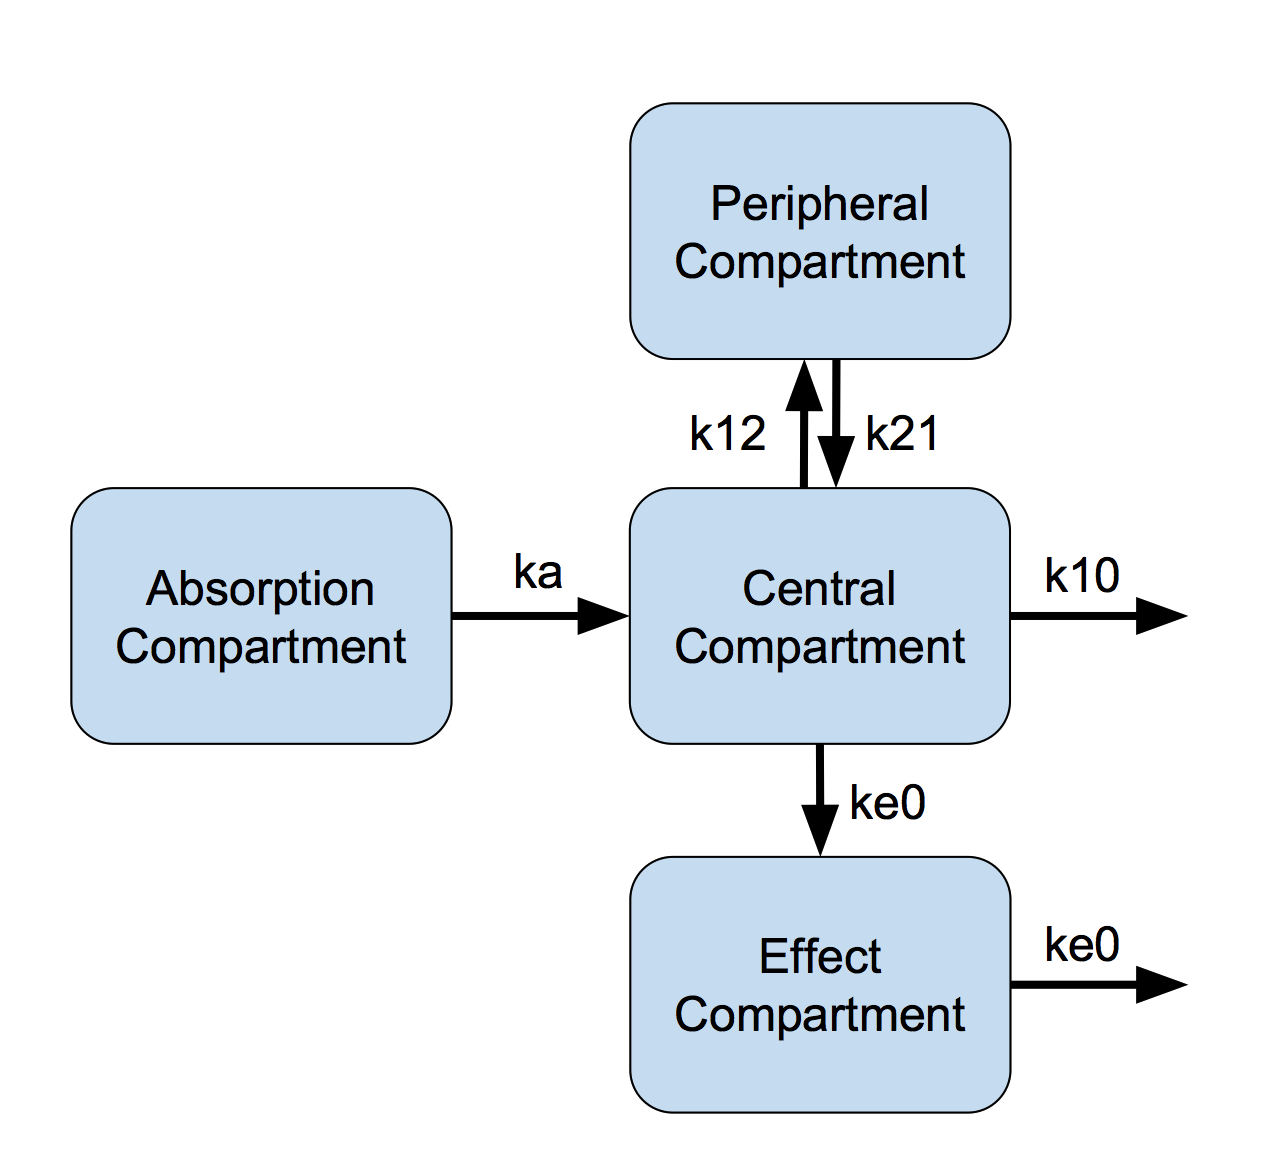
\includegraphics[width=0.5\textwidth]{./graphics/effCptModel.png}
\caption{\label{eff_model}Effect Compartment Model}
\end{figure}


\subsection{Effect Compartment Model for PD response \(R\).}
\label{sec:orgbd5a4de}
\begin{gather*}
R_{ij} \sim N\left(\widehat{R}_{ij},\sigma_{R}^2\right), \\
\widehat{R}_{ij} = \frac{E_{max}c_{eij}}{EC_{50j} + c_{eij}}, \\
c_{e\cdot j}^\prime = k_{e0j}\left(c_{\cdot j} - c_{e\cdot j}\right), \\
\log\left(EC_{50j}, k_{e0j}\right) \sim N\left(\log\left(\widehat{EC}_{50}, \widehat{k}_{e0}\right),\Omega_R\right), \\
\left(E_{max}, \widehat{EC}_{50},\widehat{k}_{e0}\right) = \left(100, 100.7, 1\right), \\
\Omega_R = \left(\begin{array}{cc} 0.2^2 & 0 \\ 0 & 0.25^2  \end{array}\right), \ \ \ \sigma_R = 10.
\end{gather*}

The PK and the PD data are simulated using the following
treatment.
\begin{itemize}
\item Phase I study
\begin{itemize}
\item Single dose and multiple doses
\item Parallel dose escalation design
\item 25 subjects per dose
\item Single doses: 5, 10, 20, and 40 mg
\item PK: plasma concentration of parent drug (\(c\))
\item PD response: Emax function of effect compartment concentration (\(R\))
\item PK and PD measured at 0.125, 0.25, 0.5, 0.75, 1, 2, 3, 4, 6, 8, 12, 18, and 24 hours
\end{itemize}
\item Phase IIa trial in patients
\begin{itemize}
\item 100 subjects
\item Multiple doses: 20 mg
\item sparse PK and PD data (3-6 samples per patient)
\end{itemize}
\end{itemize}

The model is simultaneously fitted to the PK and the PD
data. For this effect compartment model, we construct a
constant rate matrix and use \texttt{pmx\_solve\_linode}. Correct use of
Torsten requires the user pass the entire event history
(observation and dosing events) for an individual to the
function. Thus the Stan model shows the call to \texttt{pmx\_solve\_linode}
within a loop over the individual subjects rather than over
the individual observations. Note that the correlation matrix \(\rho\) does not explicitly appear
in the model, but it is used to construct \(\Omega\), which parametrizes
the PK IIV.

\begin{minted}[breaklines=true,fontsize=\footnotesize,breakanywhere=true]{stan}
data{
  int<lower = 1> nSubjects;
  int<lower = 1> nt;
  int<lower = 1> nObs;
  int<lower = 1> iObs[nObs];
  real<lower = 0> amt[nt];
  int<lower = 1> cmt[nt];
  int<lower = 0> evid[nt];
  int<lower = 1> start[nSubjects];
  int<lower = 1> end[nSubjects];
  real<lower = 0> time[nt];
  vector<lower = 0>[nObs] cObs;
  vector[nObs] respObs;
  real<lower = 0> weight[nSubjects];
  real<lower = 0> rate[nt];
  real<lower = 0> ii[nt];
  int<lower = 0> addl[nt];
  int<lower = 0> ss[nt];
}

transformed data{
  vector[nObs] logCObs = log(cObs);
  int<lower = 1> nRandom = 5;
  int nCmt = 4;
  real biovar[nCmt] = rep_array(1.0, nCmt);
  real tlag[nCmt] = rep_array(0.0, nCmt);
}

parameters{
  real<lower = 0> CLHat;
  real<lower = 0> QHat;
  real<lower = 0> V1Hat;
  real<lower = 0> V2Hat;
  //  real<lower = 0> kaHat;
  real<lower = (CLHat / V1Hat + QHat / V1Hat + QHat / V2Hat +
                sqrt((CLHat / V1Hat + QHat / V1Hat + QHat / V2Hat)^2 -
                     4 * CLHat / V1Hat * QHat / V2Hat)) / 2> kaHat; // ka > lambda_1
  real<lower = 0> ke0Hat;
  real<lower = 0> EC50Hat;
  vector<lower = 0>[nRandom] omega;
  corr_matrix[nRandom] rho;
  real<lower = 0> omegaKe0;
  real<lower = 0> omegaEC50;
  real<lower = 0> sigma;
  real<lower = 0> sigmaResp;

  // reparameterization
  vector[nRandom] logtheta_raw[nSubjects];
  real logKe0_raw[nSubjects];
  real logEC50_raw[nSubjects];
}

transformed parameters{
  vector<lower = 0>[nRandom] thetaHat;
  cov_matrix[nRandom] Omega;
  real<lower = 0> CL[nSubjects];
  real<lower = 0> Q[nSubjects];
  real<lower = 0> V1[nSubjects];
  real<lower = 0> V2[nSubjects];
  real<lower = 0> ka[nSubjects];
  real<lower = 0> ke0[nSubjects];
  real<lower = 0> EC50[nSubjects];
  matrix[nCmt, nCmt] K;
  real k10;
  real k12;
  real k21;
  row_vector<lower = 0>[nt] cHat;
  row_vector<lower = 0>[nObs] cHatObs;
  row_vector<lower = 0>[nt] respHat;
  row_vector<lower = 0>[nObs] respHatObs;
  row_vector<lower = 0>[nt] ceHat;
  matrix[nCmt, nt] x;

  matrix[nRandom, nRandom] L;
  vector[nRandom] logtheta[nSubjects];
  real logKe0[nSubjects];
  real logEC50[nSubjects];

  thetaHat[1] = CLHat;
  thetaHat[2] = QHat;
  thetaHat[3] = V1Hat;
  thetaHat[4] = V2Hat;
  thetaHat[5] = kaHat;

  Omega = quad_form_diag(rho, omega); // diag_matrix(omega) * rho * diag_matrix(omega)
  L = cholesky_decompose(Omega);

  for(j in 1:nSubjects){
    logtheta[j] = log(thetaHat) + L * logtheta_raw[j];
    logKe0[j] = log(ke0Hat) + logKe0_raw[j] * omegaKe0;
    logEC50[j] = log(EC50Hat) + logEC50_raw[j] * omegaEC50;

    CL[j] = exp(logtheta[j, 1]) * (weight[j] / 70)^0.75;
    Q[j] = exp(logtheta[j, 2]) * (weight[j] / 70)^0.75;
    V1[j] = exp(logtheta[j, 3]) * weight[j] / 70;
    V2[j] = exp(logtheta[j, 4]) * weight[j] / 70;
    ka[j] = exp(logtheta[j, 5]);
    ke0[j] = exp(logKe0[j]);
    EC50[j] = exp(logEC50[j]);

    k10 = CL[j] / V1[j];
    k12 = Q[j] / V1[j];
    k21 = Q[j] / V2[j];

    K = rep_matrix(0, nCmt, nCmt);

    K[1, 1] = -ka[j];
    K[2, 1] = ka[j];
    K[2, 2] = -(k10 + k12);
    K[2, 3] = k21;
    K[3, 2] = k12;
    K[3, 3] = -k21;
    K[4, 2] = ke0[j];
    K[4, 4] = -ke0[j];

    x[, start[j]:end[j] ] = pmx_solve_linode(time[start[j]:end[j]], amt[start[j]:end[j]],
                                             rate[start[j]:end[j]], ii[start[j]:end[j]],
                                             evid[start[j]:end[j]], cmt[start[j]:end[j]],
                                             addl[start[j]:end[j]], ss[start[j]:end[j]], K, biovar, tlag);

    cHat[start[j]:end[j]] = 1000 * x[2, start[j]:end[j]] ./ V1[j];
    ceHat[start[j]:end[j]] = 1000 * x[4, start[j]:end[j]] ./ V1[j];
    respHat[start[j]:end[j]] = 100 * ceHat[start[j]:end[j]] ./
       (EC50[j] + ceHat[start[j]:end[j]]);
  }

  cHatObs = cHat[iObs];
  respHatObs = respHat[iObs];
}

model{
  // Prior
  CLHat ~ lognormal(log(10), 0.2);
  QHat ~ lognormal(log(15), 0.2);
  V1Hat ~ lognormal(log(30), 0.2);
  V2Hat ~ lognormal(log(100), 0.2);
  kaHat ~ lognormal(log(5), 0.25);
  ke0Hat ~ lognormal(log(10), 0.25);
  EC50Hat ~ lognormal(log(1.0), 0.2);
  omega ~ normal(0, 0.2);
\end{minted}

\subsection{Results}
\label{sec:org73a9298}
We use the same diagnosis tools as for the
previous examples. Table \ref{effCptModelParms} summarises the
statistics and diagnostics of the parameters. In particular, \texttt{rhat}
for all parameters being close to 1.0 indicates convergence of the 4
chains. Figure \ref{effcpt_mcmc_density} shows the posterior density of
the parameters.

Posterior prediction check (PPC) in Figure
\ref{effcpt_ppc_5mg} - \ref{effcpt_ppc_study_2_20mg} show that the fits to the plasma concentration
are in close agreement with the data, notably for the sparse data case (phase IIa study). The fits
to the PD data (Figure \ref{effcpt_ppc_resp_5mg} - \ref{effcpt_ppc_resp_study_2_20mg}) look
reasonable considering data being more noisy so the model
produces larger credible intervals. Both the summary table and PPC
plots show that the estimated values of the
parameters are consistent with the values used to simulate the data.

\begin{table}[htbp]
\caption{\label{effCptModelParms}Summary of the MCMC simulations of the marginal posterior distributions of the model parameters for the effect compartment model example.}
\centering
\footnotesize
\begin{tabular}{r r r r r r r r r r r}
variable & mean & median & sd & mad & q5 & q95 & rhat & ess\textsubscript{bulk} & ess\textsubscript{tail}\\
\hline
CLHat & 10.121 & 10.120 & 0.195 & 0.192 & 9.797 & 10.445 & 1.007 & 319.942 & 630.619\\
QHat & 14.858 & 14.853 & 0.347 & 0.344 & 14.301 & 15.432 & 1.000 & 1106.126 & 1712.821\\
V1Hat & 34.493 & 34.516 & 1.004 & 0.995 & 32.814 & 36.086 & 1.004 & 671.777 & 1563.396\\
V2Hat & 103.269 & 103.291 & 2.876 & 2.878 & 98.568 & 108.019 & 1.002 & 1689.165 & 2580.382\\
kaHat & 1.968 & 1.969 & 0.076 & 0.074 & 1.843 & 2.087 & 1.001 & 1204.531 & 1747.427\\
ke0Hat & 1.102 & 1.100 & 0.046 & 0.045 & 1.030 & 1.180 & 1.001 & 4008.337 & 3167.030\\
EC50Hat & 99.512 & 99.542 & 2.124 & 2.098 & 95.981 & 102.987 & 1.000 & 2557.436 & 2773.519\\
omega[1] & 0.268 & 0.267 & 0.016 & 0.016 & 0.242 & 0.295 & 1.008 & 594.842 & 978.297\\
omega[2] & 0.229 & 0.228 & 0.021 & 0.021 & 0.195 & 0.264 & 1.002 & 1245.453 & 1966.911\\
omega[3] & 0.212 & 0.211 & 0.029 & 0.029 & 0.165 & 0.261 & 1.005 & 623.820 & 1692.248\\
omega[4] & 0.263 & 0.262 & 0.026 & 0.026 & 0.221 & 0.306 & 1.002 & 1396.611 & 2260.425\\
omega[5] & 0.272 & 0.271 & 0.036 & 0.035 & 0.217 & 0.335 & 1.008 & 293.132 & 728.867\\
rho[1,2] & 0.197 & 0.200 & 0.100 & 0.101 & 0.029 & 0.360 & 1.003 & 1322.261 & 1955.862\\
rho[1,3] & -0.161 & -0.161 & 0.122 & 0.121 & -0.361 & 0.042 & 1.001 & 1609.160 & 2270.515\\
rho[1,4] & -0.101 & -0.105 & 0.107 & 0.107 & -0.270 & 0.083 & 1.001 & 1685.591 & 2353.498\\
rho[1,5] & 0.016 & 0.015 & 0.128 & 0.128 & -0.192 & 0.226 & 1.000 & 2039.767 & 2939.988\\
rho[2,3] & 0.091 & 0.092 & 0.144 & 0.148 & -0.143 & 0.328 & 1.008 & 718.187 & 1550.836\\
rho[2,4] & 0.186 & 0.190 & 0.125 & 0.125 & -0.025 & 0.384 & 1.005 & 948.704 & 1819.199\\
rho[2,5] & 0.146 & 0.145 & 0.157 & 0.161 & -0.111 & 0.402 & 1.003 & 626.620 & 1546.157\\
rho[3,4] & 0.815 & 0.827 & 0.093 & 0.094 & 0.646 & 0.947 & 1.010 & 309.098 & 736.635\\
rho[3,5] & -0.318 & -0.323 & 0.219 & 0.228 & -0.678 & 0.055 & 1.016 & 200.806 & 607.958\\
rho[4,5] & -0.295 & -0.299 & 0.161 & 0.162 & -0.551 & -0.019 & 1.008 & 546.998 & 1151.092\\
omegaKe0 & 0.265 & 0.265 & 0.047 & 0.047 & 0.188 & 0.346 & 1.001 & 1731.276 & 2049.892\\
omegaEC50 & 0.216 & 0.216 & 0.020 & 0.020 & 0.182 & 0.249 & 1.001 & 1599.567 & 1844.056\\
sigma & 0.099 & 0.099 & 0.002 & 0.002 & 0.095 & 0.103 & 1.002 & 1726.283 & 2836.027\\
sigmaResp & 10.165 & 10.166 & 0.198 & 0.198 & 9.844 & 10.495 & 1.002 & 4788.527 & 2923.203\\
\end{tabular}
\end{table}

\begin{figure}[htbp]
\centering
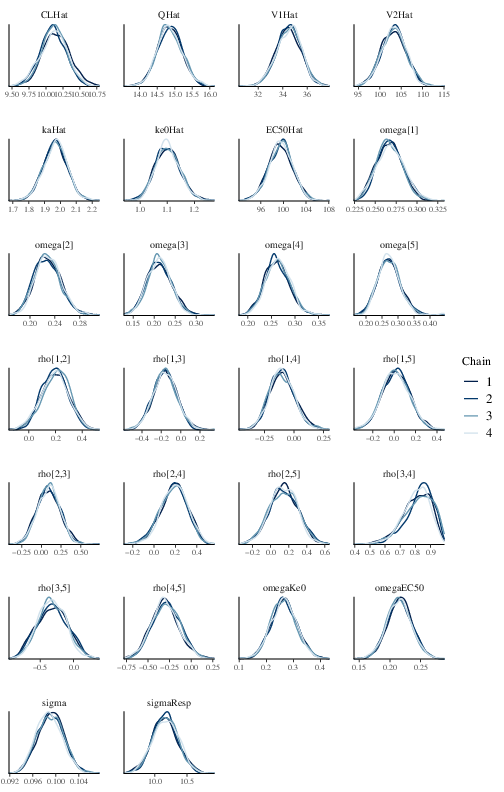
\includegraphics[width=0.8\linewidth]{../example-models/effCpt/density.pdf}
\caption{\label{effcpt_mcmc_density}Posterior marginal densities of the model parameters of the effect compartment model.}
\end{figure}

\begin{figure}[htbp]
\centering
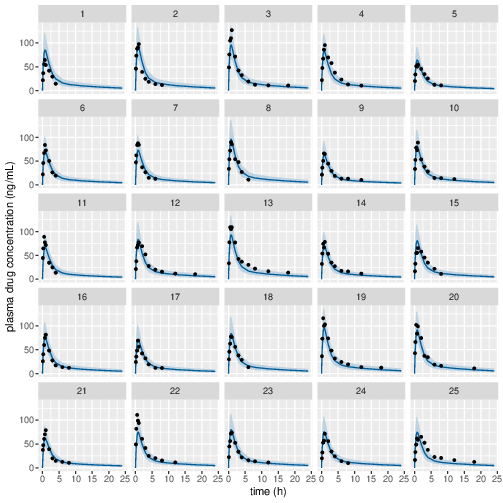
\includegraphics[width=\linewidth]{../example-models/effCpt/ppc_study_1_5mg.pdf}
\caption{\label{effcpt_ppc_5mg}Predicted (90\% credible interval and median) and observed individual plasma drug concentrations in study 1 (5mg dose).}
\end{figure}

\begin{figure}[htbp]
\centering
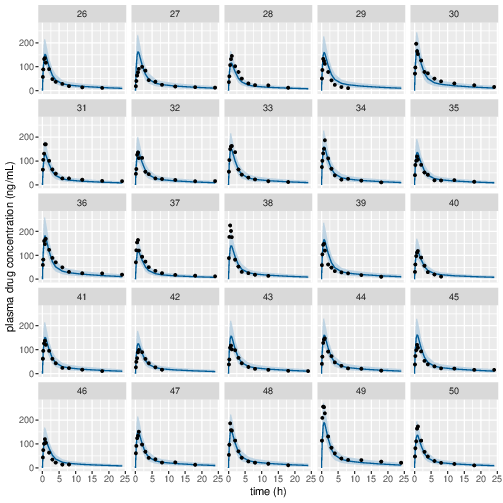
\includegraphics[width=\linewidth]{../example-models/effCpt/ppc_study_1_10mg.pdf}
\caption{\label{effcpt_ppc_10mg}Predicted (90\% credible interval and median) and observed individual plasma drug concentrations in study 1 (10mg dose).}
\end{figure}

\begin{figure}[htbp]
\centering
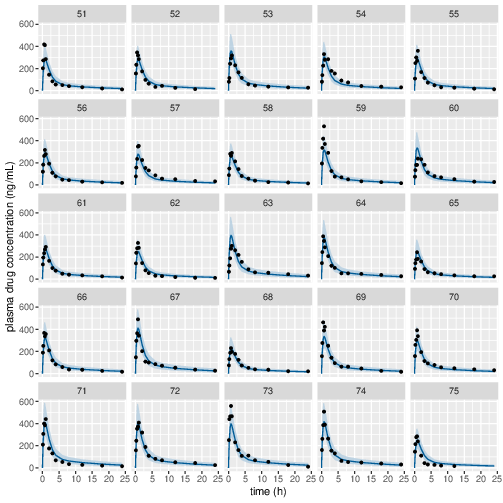
\includegraphics[width=\linewidth]{../example-models/effCpt/ppc_study_1_20mg.pdf}
\caption{\label{effcpt_ppc_20mg}Predicted (90\% credible interval and median) and observed individual plasma drug concentrations in study 1 (20mg dose).}
\end{figure}

\begin{figure}[htbp]
\centering
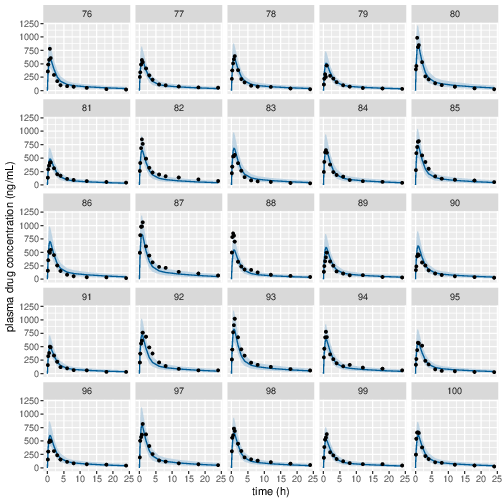
\includegraphics[width=\linewidth]{../example-models/effCpt/ppc_study_1_40mg.pdf}
\caption{\label{effcpt_ppc_40mg}Predicted (90\% credible interval and median) and observed individual plasma drug concentrations in study 1 (40mg dose).}
\end{figure}

\begin{figure}[htbp]
\centering
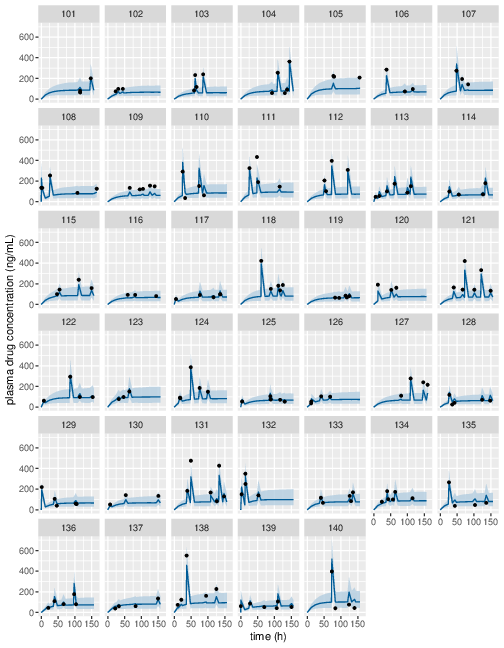
\includegraphics[width=\linewidth]{../example-models/effCpt/ppc_study_2_20mg.pdf}
\caption{\label{effcpt_ppc_study_2_20mg}Predicted (90\% credible interval and median) and observed individual plasma drug concentrations in study 2 (first 40 subjects).}
\end{figure}

\begin{figure}[htbp]
\centering
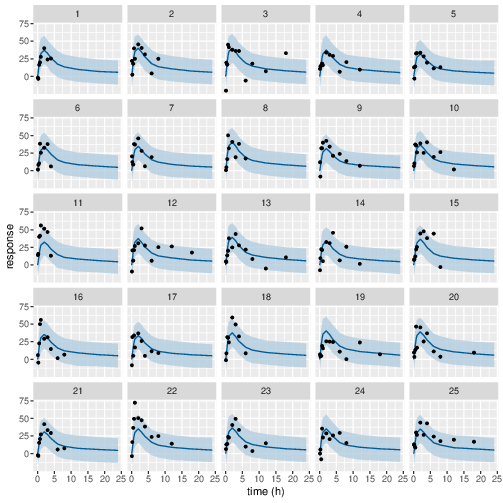
\includegraphics[width=\linewidth]{../example-models/effCpt/ppc_study_1_5mg_resp.pdf}
\caption{\label{effcpt_ppc_resp_5mg}Predicted (90\% credible interval and median) and observed individual PD response in study 1 (5mg dose).}
\end{figure}

\begin{figure}[htbp]
\centering
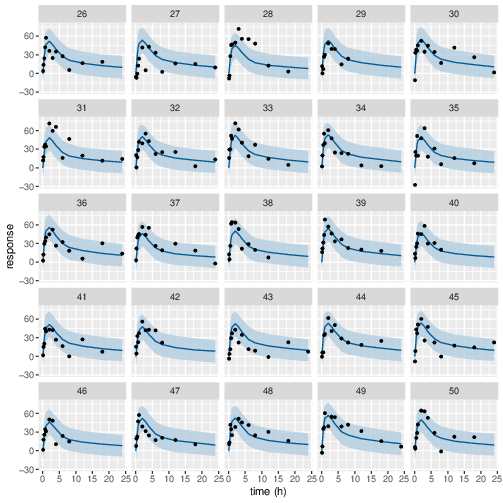
\includegraphics[width=\linewidth]{../example-models/effCpt/ppc_study_1_10mg_resp.pdf}
\caption{\label{effcpt_ppc_resp_10mg}Predicted (90\% credible interval and median) and observed individual PD response in study 1 (10mg dose).}
\end{figure}

\begin{figure}[htbp]
\centering
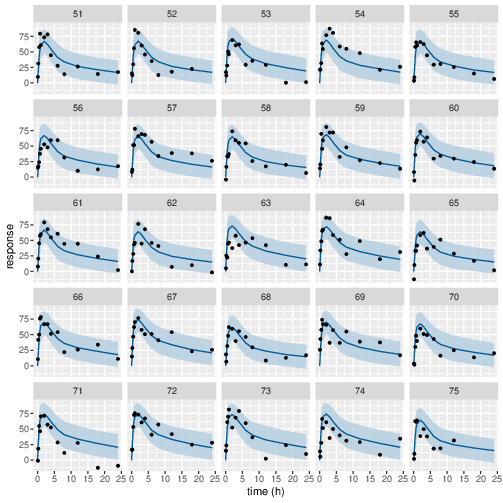
\includegraphics[width=\linewidth]{../example-models/effCpt/ppc_study_1_20mg_resp.pdf}
\caption{\label{effcpt_ppc_resp_20mg}Predicted (90\% credible interval and median) and observed individual PD response in study 1 (20mg dose).}
\end{figure}

\begin{figure}[htbp]
\centering
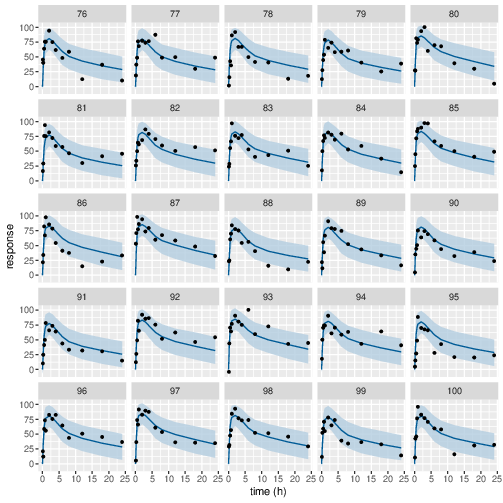
\includegraphics[width=\linewidth]{../example-models/effCpt/ppc_study_1_40mg_resp.pdf}
\caption{\label{effcpt_ppc_resp_40mg}Predicted (90\% credible interval and median) and observed individual PD response in study 1 (40mg dose).}
\end{figure}

\begin{figure}[htbp]
\centering
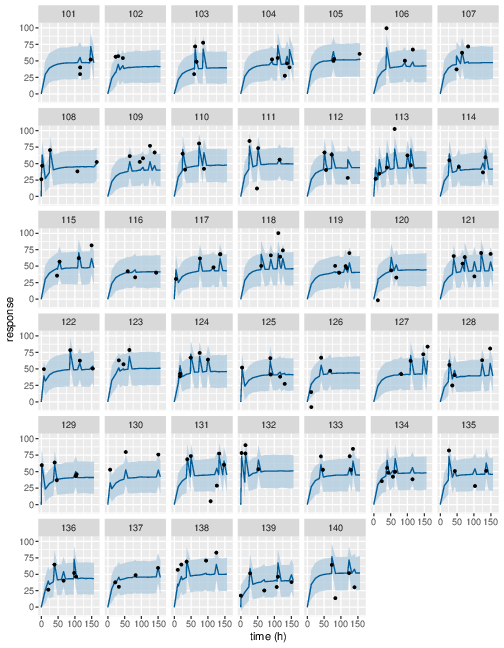
\includegraphics[width=\linewidth]{../example-models/effCpt/ppc_study_2_20mg_resp.pdf}
\caption{\label{effcpt_ppc_resp_study_2_20mg}Predicted (90\% credible interval and median) and observed individual PD response in study 2 (first 40 subjects).}
\end{figure}

\section{Friberg-Karlsson Semi-Mechanistic Population Model}
\label{sec:org830b60b}
We now return to the example of \ref{sec:fk_model} and extend
it to a population model. While we recommend using the coupled
solver, and this time we solve it using group solver. We leave it
as an exercise to the reader to rewrite the model with
coupled solver.

\subsection{Friberg-Karlsson Population Model for drug-induced myelosuppression (\(ANC\))}
\label{sec:org1cc1dab}
\begin{gather*}
\log(ANC_{ij}) \sim N(Circ_{ij}, \sigma^2_{ANC}), \\
\log\left(MTT_j, Circ_{0j}, \alpha_j\right) \sim N\left(\log\left(\widehat{MTT}, \widehat{Circ_0}, \widehat{\alpha}\right), \Omega_{ANC}\right), \\
\left(\widehat{MTT}, \widehat{Circ}_0,\widehat{\alpha}, \gamma \right) = \left(125, 5, 2, 0.17\right), \\
\Omega_{ANC} = \left(\begin{array}{ccc} 0.2^2 & 0 & 0 \\ 0 & 0.35^2 & 0 \\ 0 & 0 & 0.2^2 \end{array}\right), \\
\sigma_{ANC} = 0.1, \\
\Omega_{PK} = \left(\begin{array}{ccccc} 0.25^2 & 0 &a 0 & 0 & 0 \\ 0 & 0.4^2 & 0 & 0 & 0 \\
0 & 0 & 0.25^2 & 0 & 0 \\ 0 & 0 & 0 & 0.4^2 & 0 \\ 0 & 0 & 0 & 0 & 0.25^2  \end{array}\right)
\end{gather*}
The PK and the PD data are simulated using the following treatment.
\begin{itemize}
\item Phase IIa trial in patients
\begin{itemize}
\item Multiple doses: 80,000 mg
\item Parallel dose escalation design
\item 15 subjects
\item PK: plasma concentration of parent drug (\(c\))
\item PD response: Neutrophil count (\(ANC\))
\item PK measured at 0.083, 0.167, 0.25, 0.5, 0.75, 1, 2, 3, 4, 6, 8, 12, 18, and 24 hours
\item PD measured once every two days for 28 days.
\end{itemize}
\end{itemize}

Once again, we simultaneously fit the model to the PK and the PD
data. It pays off to construct informative priors. For instance, we could
fit the PK data first, as was done in  example 1, and get informative
priors on the PK parameters. The PD parameters are drug independent,
so we can use information from the neutropenia literature. In this
example, we choose to use strongly informative priors on both PK and PD
parameters.

The ODE is defined as
\begin{minted}[breaklines=true,fontsize=\footnotesize,breakanywhere=true]{stan}
functions{
    vector twoCptNeutModelODE(real t, vector x, array[] real parms, array[] real rdummy, array[] int idummy){
    real k10;
    real k12;
    real k21;
    real CL;
    real Q;
    real V1;
    real V2;
    real ka;
    real mtt;
    real circ0;
    real gamma;
    real alpha;
    real ktr;
    vector[8] dxdt;
    real conc;
    real EDrug;
    real transit1;
    real transit2;
    real transit3;
    real circ;
    real prol;

    CL = parms[1];
    Q = parms[2];
    V1 = parms[3];
    V2 = parms[4];
    ka = parms[5];
    mtt = parms[6];
    circ0 = parms[7];
    gamma = parms[8];
    alpha = parms[9];

    k10 = CL / V1;
    k12 = Q / V1;
    k21 = Q / V2;

    ktr = 4 / mtt;

    dxdt[1] = -ka * x[1];
    dxdt[2] = ka * x[1] - (k10 + k12) * x[2] + k21 * x[3];
    dxdt[3] = k12 * x[2] - k21 * x[3];
    conc = x[2]/V1;
    EDrug = alpha * conc;
    // x[4], x[5], x[6], x[7] and x[8] are differences from circ0.
    prol = x[4] + circ0;
    transit1 = x[5] + circ0;
    transit2 = x[6] + circ0;
    transit3 = x[7] + circ0;
    circ = fmax(machine_precision(), x[8] + circ0); // Device for implementing a modeled
                                                    // initial condition
    dxdt[4] = ktr * prol * ((1 - EDrug) * ((circ0 / circ)^gamma) - 1);
    dxdt[5] = ktr * (prol - transit1);
    dxdt[6] = ktr * (transit1 - transit2);
    dxdt[7] = ktr * (transit2 - transit3);
    dxdt[8] = ktr * (transit3 - circ);

    return dxdt;
  }
}
\end{minted}

We use the \texttt{pmx\_solve\_group\_rk45} function to
solve the entire population's events.
\begin{minted}[breaklines=true,fontsize=\footnotesize,breakanywhere=true]{stan}
transformed parameters{
  row_vector[nt] cHat;
  vector[nObsPK] cHatObs;
  row_vector[nt] neutHat;
  vector[nObsPD] neutHatObs;
  matrix[8, nt] x;
  real<lower = 0> parms[nSubjects, nTheta]; // The [1] indicates the parameters are constant

  // variables for Matt's trick
  vector<lower = 0>[nIIV] thetaHat;
  matrix<lower = 0>[nSubjects, nIIV] thetaM;

  // Matt's trick to use unit scale
  thetaHat[1] = CLHat;
  thetaHat[2] = QHat;
  thetaHat[3] = V1Hat;
  thetaHat[4] = V2Hat;
  thetaHat[5] = mttHat;
  thetaHat[6] = circ0Hat;
  thetaHat[7] = alphaHat;
  thetaM = (rep_matrix(thetaHat, nSubjects) .*
             exp(diag_pre_multiply(omega, L * etaStd)))';

  for(i in 1:nSubjects) {
    parms[i, 1] = thetaM[i, 1] * (weight[i] / 70)^0.75; // CL
    parms[i, 2] = thetaM[i, 2] * (weight[i] / 70)^0.75; // Q
    parms[i, 3] = thetaM[i, 3] * (weight[i] / 70); // V1
    parms[i, 4] = thetaM[i, 4] * (weight[i] / 70); // V2
    parms[i, 5] = kaHat; // ka
    parms[i, 6] = thetaM[i, 5]; // mtt
    parms[i, 7] = thetaM[i, 6]; // circ0
    parms[i, 8] = gamma;
    parms[i, 9] = thetaM[i, 7]; // alpha
  }

  /* group solver */
  x = pmx_solve_group_rk45(twoCptNeutModelODE, 8, len,
                           time, amt, rate, ii, evid, cmt, addl, ss,
                           parms,
                           1e-6, 1e-6, 500);

  for(i in 1:nSubjects) {
    cHat[start[i]:end[i]] = x[2, start[i]:end[i]] / parms[i, 3]; // divide by V1
    neutHat[start[i]:end[i]] = x[8, start[i]:end[i]] + parms[i, 7]; // Add baseline
  }

  for(i in 1:nObsPK) cHatObs[i] = cHat[iObsPK[i]];
  for(i in 1:nObsPD) neutHatObs[i] = neutHat[iObsPD[i]];
}
\end{minted}

This allows us to use within-chain paralleleisation to reduce
simulation time. When run from cmdstan, each MPI run generates one
chain, and we use 4 MPI runs to generate 4 chains.
\begin{minted}[breaklines=true,fontsize=\footnotesize,breakanywhere=true]{bash}
# chain 1
mpiexec -n nproc ./FribergKarlsson sample adapt delta=0.95 data file=fribergkarlsson.data.R init=fribergkarlsson.init.R random seed=8765 id=1 output file=output.1.csv
# chain 2
mpiexec -n nproc ./FribergKarlsson sample adapt delta=0.95 data file=fribergkarlsson.data.R init=fribergkarlsson.init.R random seed=8765 id=2 output file=output.2.csv
# chain 3
mpiexec -n nproc ./FribergKarlsson sample adapt delta=0.95 data file=fribergkarlsson.data.R init=fribergkarlsson.init.R random seed=8765 id=3 output file=output.3.csv
# chain 4
mpiexec -n nproc ./FribergKarlsson sample adapt delta=0.95 data file=fribergkarlsson.data.R init=fribergkarlsson.init.R random seed=8765 id=4 output file=output.4.csv
\end{minted}

\subsection{Results}
\label{sec:orgecf35b4}
Table \ref{FkpopModelParms} summarizes the sampling and some diagnostics output.
estimation reflects the real value of the parameters (Table \ref{FkpopModelParms} and Figure \ref{fkpop_mcmc_density}.
Similar to the previous example, PPCs shown in Figure \ref{fkpop_ppc_pk}
and \ref{fkpop_ppc_pd} indicate the model is a good fit.

\begin{table}[htbp]
\caption{\label{FkpopModelParms}Summary of the MCMC simulations of the marginal posterior distributions of the model parameters for the Friberg-Karlsson population model example.}
\centering
\footnotesize
\begin{tabular}{r r r r r r r r r r r}
variable & mean & median & sd & mad & q5 & q95 & rhat & ess\textsubscript{bulk} & ess\textsubscript{tail}\\
\hline
CLHat & 9.539 & 9.535 & 0.522 & 0.487 & 8.692 & 10.401 & 1.006 & 971.369 & 1655.449\\
QHat & 15.401 & 15.386 & 1.018 & 1.000 & 13.742 & 17.090 & 1.000 & 2263.843 & 2447.006\\
V1Hat & 37.396 & 37.360 & 2.244 & 2.228 & 33.762 & 41.058 & 1.001 & 1936.476 & 2372.815\\
V2Hat & 101.698 & 101.394 & 6.503 & 6.119 & 91.529 & 112.538 & 1.001 & 2580.227 & 2592.925\\
kaHat & 1.997 & 1.997 & 0.074 & 0.074 & 1.873 & 2.115 & 1.001 & 7056.877 & 2993.406\\
mttHat & 113.681 & 113.204 & 11.506 & 10.910 & 95.807 & 133.514 & 1.001 & 4255.900 & 3269.646\\
circ0Hat & 4.760 & 4.752 & 0.241 & 0.229 & 4.375 & 5.163 & 1.002 & 3774.920 & 2783.663\\
omega[1] & 0.223 & 0.217 & 0.047 & 0.042 & 0.160 & 0.307 & 1.000 & 1751.864 & 2235.607\\
omega[2] & 0.339 & 0.329 & 0.073 & 0.067 & 0.239 & 0.473 & 1.001 & 2363.843 & 2607.056\\
omega[3] & 0.264 & 0.256 & 0.057 & 0.051 & 0.186 & 0.367 & 1.002 & 2128.660 & 2018.425\\
omega[4] & 0.257 & 0.249 & 0.056 & 0.051 & 0.182 & 0.361 & 1.003 & 2293.877 & 2937.673\\
omega[5] & 0.177 & 0.169 & 0.112 & 0.118 & 0.019 & 0.376 & 1.000 & 1550.483 & 2045.025\\
omega[6] & 0.188 & 0.183 & 0.044 & 0.041 & 0.127 & 0.269 & 1.000 & 2377.698 & 2965.713\\
omega[7] & 0.409 & 0.394 & 0.256 & 0.259 & 0.045 & 0.865 & 1.003 & 1386.987 & 2015.873\\
gamma & 0.171 & 0.168 & 0.035 & 0.033 & 0.121 & 0.235 & 1.000 & 8809.668 & 3189.676\\
sigma & 0.097 & 0.096 & 0.003 & 0.003 & 0.093 & 0.101 & 1.002 & 5436.508 & 2899.706\\
sigmaNeut & 0.106 & 0.105 & 0.012 & 0.011 & 0.088 & 0.127 & 1.000 & 2809.059 & 3031.605\\
alphaHat & 2.24e-4 & 2.19e-4 & 3.97e-05 & 3.80e-05 & 1.66e-4 & 2.96e-4 & 1.000 & 5138.105 & 2807.328\\
\end{tabular}
\end{table}

\begin{figure}[htbp]
\centering
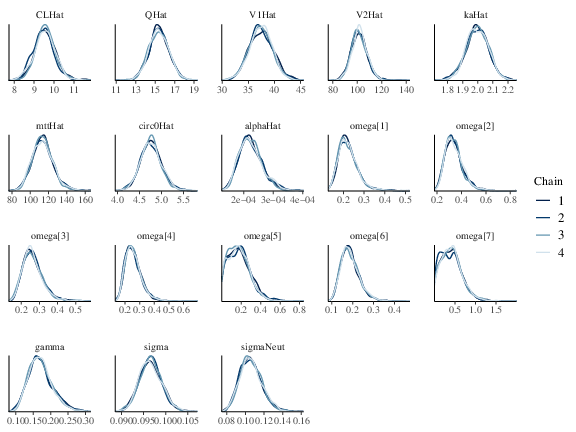
\includegraphics[width=0.8\linewidth]{../example-models/FribergKarlsson/density.pdf}
\caption{\label{fkpop_mcmc_density}Posterior marginal densities of the model parameters of the Friberg-Karlsson population model.}
\end{figure}

\begin{figure}[htbp]
\centering
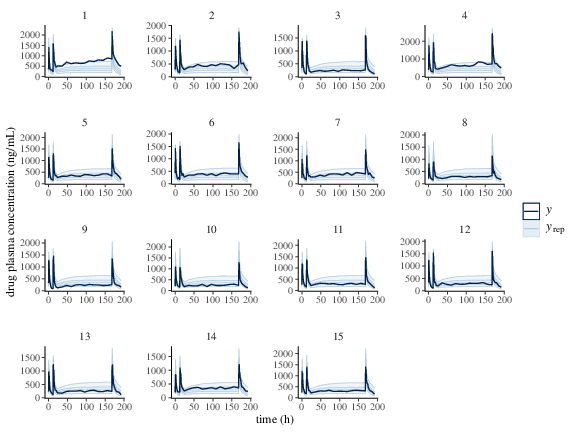
\includegraphics[width=0.8\linewidth]{../example-models/FribergKarlsson/ppc_pk.pdf}
\caption{\label{fkpop_ppc_pk}Predicted (50\%, 90\% credible interval and median) and observed individual drug plasma concentration.}
\end{figure}

\begin{figure}[htbp]
\centering
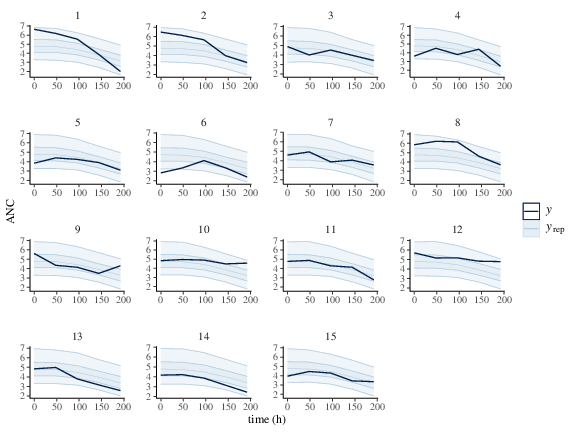
\includegraphics[width=0.8\linewidth]{../example-models/FribergKarlsson/ppc_pd.pdf}
\caption{\label{fkpop_ppc_pd}Predicted (50\%, 90\% credible interval and median) and observed individual Neutrophil counts.}
\end{figure}

\appendix
\chapter*{Compiling constants}
\label{sec:org9e915c4}
Several constants are used in Torsten's makefile. These constants can
be used in \texttt{cmdstan/make/local} file, or use \texttt{set\_make\_local} command
in \texttt{cmdstanr}.
\begin{itemize}
\item \texttt{TORSTEN\_MPI=1} turns on within-chain parallelsation of MPI-enable
functions. To use this option one must also point
\texttt{TBB\_CXX\_TYPE} to proper C compiler. See also Section \ref{sec:org6157bc2} and \ref{sec:orge34552c}.
\item \texttt{TORSTEN\_CVS\_JAC\_AD=1} makes BDF and Adams
integrator use Stan's automatic differentiation to calculate
Jacobian matrix in nonlinear solver \cite{hindmarsh_cvodes_2020}.
\end{itemize}

\printindex

\backmatter

\label{bibliographystyle link}
\bibliographystyle{unsrt}

\label{bibliography link}
\bibliography{torsten}
\end{document}
